\documentclass[letterpaper,11pt]{article}

\usepackage[spanish,es-tabla]{babel}
\usepackage[T1]{fontenc}
\usepackage[left=2cm,right=2cm,top=2cm,bottom=2cm]{geometry}
\usepackage{amsmath}
\usepackage{array}
\usepackage{caption}
\usepackage{color}
\usepackage{float}
\usepackage{graphicx}
\usepackage{hyperref}
\usepackage{parskip}
\usepackage{listings}
\usepackage{xcolor}
\usepackage[spanish]{babel}


\setlength{\parindent}{0pt}
\renewcommand{\arraystretch}{1.3}

\lstdefinestyle{MatlabStyle}{
  language=Matlab,
  basicstyle=\small\ttfamily,
  keywordstyle=\color{blue},
  identifierstyle=\color{black},
  commentstyle=\color{teal}\textit,
  stringstyle=\color{red},
  numbers=left,
  numberstyle=\tiny\color{gray},
  stepnumber=1,
  numbersep=10pt,
  showspaces=false,
  showtabs=false,
  showstringspaces=false,
  extendedchars=true,
  breaklines=true,
  breakatwhitespace=true,
  tabsize=2,
  frame=single,
  framerule=1pt,
  rulecolor=\color{gray},
  backgroundcolor=\color{lightgray!10},
  captionpos=b,
  abovecaptionskip=5pt,
  belowcaptionskip=5pt,
  xleftmargin=10pt,
  xrightmargin=10pt,
  aboveskip=10pt,
  belowskip=10pt,
  rulesepcolor=\color{orange}
}

\begin{document}
    \begin{titlepage}
        \centering
        \begin{tabular}{@{}m{0.2\textwidth}@{}m{0.6\textwidth}@{}m{0.2\textwidth}@{}}
            \centering\raisebox{-\depth}{
\includegraphics[width=2.5cm, height=3cm]{assets/ipn (1).jpeg}} & % Tamaño fijo y alineación
            \centering \textsc{\textbf{\LARGE Instituto Politécnico Nacional}} & 
            \centering\raisebox{-\depth}{
\includegraphics[width=2.5cm, height=3cm]{assets/escom (1).jpeg}} \\ % Tamaño fijo y   alineación
        \end{tabular}
    
        \vspace{2cm} % Espacio después de los logotipos y el nombre
    
        {\LARGE Procesamiento de Señales}\\[1.5cm]
    
        {\fontsize{20pt}{20pt}\selectfont \textbf{Proyecto}\\[0.5 cm] Título del proyecto }\\[3cm]
        
        \begin{tabular}{@{\hspace{0.5cm}}p{0.45\textwidth}@{\hspace{0.5cm}}p{0.45\textwidth}@{}}
            \textbf{INTEGRANTES:} & \hfill \textbf{GRUPO 5BV1} \\[0.3cm]
            Gutiérrez Sánchez Angélica   & \hfill Miguel Ángel Castillo Martínez\\[0.2cm]
            Hernández Jiménez Erick Yael  & \hfill 15 de junio de 2025
        \end{tabular}
        \end{titlepage}

    \tableofcontents % Tabla de contenidos

    \newpage 

    \section{Introducción}
        \subsection{Descripción del problema}
            El estudio del entorno magnético de Venus representa un reto científico significativo, debido a la ausencia de un campo magnético intrínseco y a la fuerte influencia del viento solar sobre su ionosfera. Esta interacción genera una magnetosfera inducida altamente variable, cuya estructura y dinámica aún no se comprenden del todo. A pesar de los avances proporcionados por misiones como Venus Express y, más recientemente, Solar Orbiter, el análisis fino de los datos obtenidos por instrumentos como el magnetómetro MAG requiere un tratamiento riguroso de señales que presentan ruido, picos anómalos y posibles errores de medición \cite{zhan2006}.

            En particular, las señales de campo magnético medidas a bordo de Venus Express contienen componentes espurias que pueden deberse a interferencias de la propia nave, errores de calibración o condiciones de entorno espacial extremas. Estos errores dificultan la interpretación científica del entorno magnético venusiano, sobre todo cuando se pretende analizar fenómenos sutiles como estructuras de plasma o variaciones inducidas por tormentas solares \cite{esa}.

            El análisis y tratamiento adecuado de estas señales, mediante técnicas de procesamiento como filtrado y comparación entre sensores redundantes (por ejemplo, el uso combinado de los sistemas BIS y BOS), resulta esencial para obtener una representación fiable del campo magnético ambiental de Venus. Este proyecto se enfoca en dicha tarea, abordando tanto la identificación de picos anómalos como el diseño de filtros adecuados para depurar las lecturas y permitir un análisis físico consistente.

        \subsection{Objetivos}
            \subsubsection{Objetivo general}

            Analizar y procesar las señales del magnetómetro MAG de la misión Venus Express para calcular y caracterizar la magnitud del campo magnético inducido (BOST), evaluando su estructura mediante técnicas de tratamiento de señales y comparándola con los datos de referencia proporcionados por la Agencia Espacial Europea (ESA).
            
        
            \subsubsection{Objetivos específicos}
                \begin{itemize}
                    \item Adquirir y explorar los datos magnéticos proporcionados por el magnetómetro MAG de la misión Venus Express, especialmente los correspondientes a la familia BOS.
                    
                    \item Implementar técnicas de filtrado y limpieza sobre las señales crudas BOSX, BOSY y BOSZ para mitigar ruido instrumental y picos anómalos.
                    
                    \item Calcular la magnitud total del campo magnético inducido (BOST) a partir de las componentes filtradas del vector magnético.

                    \item Comparar la señal BOST procesada con la señal de referencia publicada por la Agencia Espacial Europea para validar la calidad del procesamiento.

                    \item Interpretar los resultados en el contexto físico del entorno magnético de Venus y su interacción con el viento solar.
                \end{itemize}

\newpage
        \subsection{Organización del documento}
            Primero, el marco teórico aborda el fenómeno estudiado por la misión \textit{Venus Express} en Venus, así como detalles relevantes de esta misión, incluyendo los conocimientos esperados, su instrumentación y los sistemas de referencia.

            Posteriormente, se detalla la metodología empleada, la cual incluye la recolección, selección y visualización de datos, un análisis de los filtros utilizados para el tratamiento de la señal recibida y el cálculo de la magnitud de las tres señales seleccionadas.

            Finalmente, se presentarán los resultados obtenidos tras la aplicación de los filtros seleccionados, y en las conclusiones, se realizará una evaluación crítica del producto final.

\newpage
    % \newpage
    \section{Marco Teórico}
        % Agregaría una breve introducción aquí
        \subsection{Entorno espacial de Venus}
            % Y otra breve introducción acá
            \subsubsection{Campo magnético inducido}
                Venus, a diferencia de la Tierra, no posee un campo magnético intrínseco generado por un núcleo en rotación. En cambio, genera un campo magnético inducido como consecuencia de la interacción entre el viento solar y la ionosfera del planeta, una región cargada de iones y electrones. Este campo inducido no está anclado internamente, por lo que es inestable y altamente variable, especialmente sensible a las condiciones del viento solar \cite{nasa2025}.


                La misión \textit{Solar Orbiter}, desarrollada por la Agencia Espacial Europea (ESA) en colaboración con la NASA, ha contribuido recientemente a la documentación del campo magnético inducido de Venus. Sus observaciones han confirmado que el entorno magnético del planeta suele ser débil, con intensidades típicas entre 0.1 nT y 50 nT, alcanzando valores de hasta 200 nT en condiciones extremas \cite{solarorbiter2021}.

            \subsubsection{Ionosfera}

                La ionosfera de Venus es una región de su atmósfera superior, ubicada aproximadamente entre los 120 km y 300 km de altitud, donde la radiación ultravioleta solar ioniza los gases atmosféricos. Esto genera una capa rica en iones y electrones libres, con alta conductividad eléctrica, lo cual la convierte en una región clave para la generación del campo magnético inducido \cite{patzold2007}.

                En el caso de Venus, la ionosfera no se encuentra protegida por un campo magnético interno como en la Tierra, sino que interactúa directamente con el viento solar. Esta interacción genera corrientes inducidas que envuelven al planeta y dan lugar a una magnetocola extendida en la dirección opuesta al flujo solar, semejante a la de un cometa. La estructura de esta región varía significativamente según la densidad local de iones y la intensidad del viento solar incidente \cite{nasa2025}.


        \subsection{Misión Venus Express}

            \subsubsection{Órbita operativa}

                Venus Express fue diseñada para estudiar el planeta desde una trayectoria que maximizara la recolección de datos científicos. Para lograrlo, se eligió una órbita altamente elíptica que permitía a la nave acercarse hasta unos 250 km de la superficie en su punto más bajo (pericentro) y alejarse hasta 66,000 km en su punto más alto (apocentro). Esta gran variación en altitud permitía observar detalles locales durante el acercamiento, y realizar estudios de gran escala cuando se encontraba lejos \cite{esaorbita}.

                La inclinación de casi 90° con respecto al ecuador del planeta permitía que la nave recorriera desde el polo norte hasta el polo sur, cubriendo todas las regiones latitudinales. Además, al completar cada recorrido en 24 horas terrestres, Venus Express mantenía una ventana de comunicación constante con la Tierra y permitía observaciones regulares en las mismas franjas horarias. Durante un día sideral de Venus (243 días terrestres), se logró cubrir todas las longitudes del planeta. En el primer ciclo completo, se priorizó una cobertura global; en el segundo, se profundizó en fenómenos específicos identificados previamente, permitiendo estudios comparativos y de seguimiento \cite{esaorbita}.

                Aunque el recorrido fue cuidadosamente diseñado, no era completamente estable. La atracción gravitatoria del Sol afectaba su trayectoria, elevando gradualmente el punto de mayor cercanía; para mantener la eficacia de la misión, se realizaban ajustes periódicos mediante propulsores.
            

        
            \subsubsection{Instrumentación}
                La sonda Venus Express estaba equipada con siete instrumentos científicos diseñados para estudiar la atmósfera, la ionosfera y el entorno espacial de Venus. Uno de los instrumentos clave fue el magnetómetro (MAG), encargado de registrar variaciones en el campo magnético \cite{esa}. Su funcionamiento y análisis detallado se desarrolla mas adelante.

                \begin{itemize}
                    \item \textit{ASPERA-4} (Analyzer of Space Plasmas and Energetic Atoms): Analiza iones, electrones y átomos neutros para estudiar la interacción del viento solar con la atmósfera y los mecanismos de pérdida atmosférica.
                    \item \textit{SPICAV} (Spectroscopy for Investigation of Characteristics of the Atmosphere of Venus): Espectrómetro ultravioleta e infrarrojo que analiza la estructura vertical de la atmósfera, la composición química y fenómenos como emisiones aurorales.
                    \item \textit{VIRTIS} (Visible and Infrared Thermal Imaging Spectrometer): Captura imágenes espectrales en el visible e infrarrojo para estudiar la dinámica atmosférica, distribución de temperatura y nubes, y posibles indicios de vulcanismo.
                    \item \textit{VeRa} (Venus Radio Science): Utiliza radio ocultación para obtener perfiles verticales de temperatura, densidad y presión, tanto en la atmósfera como en la ionosfera.

                    \item \textit{VMC} (Venus Monitoring Camera): Cámara multicanal (UV, visible e IR) que monitorea fenómenos meteorológicos globales, como movimientos de nubes y vórtices polares.

                    \item \textit{PFS} (Planetary Fourier Spectrometer): Diseñado para sondeos infrarrojos entre 0.9 y 45~$\mu$m, pero presentó fallas técnicas que limitaron su uso durante la misión.
                \end{itemize}
\vspace{0.2cm}
                Cabe destacar que, aunque el magnetómetro MAG opera de forma autónoma, su interpretación se enriquece al correlacionarse con otros instrumentos de la misión. Por ejemplo, ASPERA-4 proporciona información sobre partículas cargadas que complementa la detección de variaciones en el campo magnético; SPICAV y VeRa permiten caracterizar la estructura de la atmósfera y la ionosfera, fundamentales para entender las condiciones bajo las cuales se generan las perturbaciones magnéticas. Así, el análisis del campo magnético inducido de Venus requiere una visión integral basada en datos multisensor.

            \subsubsection{MAG (Magnetómetro)}
                El instrumento \textit{MAG} mide el vector del campo magnético con una frecuencia de muestreo de hasta 128~Hz, y también proporciona versiones a menor resolución, como los registros a 1~Hz, que resultan especialmente útiles para análisis de larga duración o estudios globales. Utiliza dos sensores triaxiales tipo fluxgate cuya configuración dual permite separar los efectos del campo magnético ambiental del espacio de las interferencias generadas por la propia nave espacial \cite{esa2}.


                Ambos sensores fluxgate, de bajo peso y bajo consumo energético, consisten en dos núcleos anulares simples (ringcore) que miden el campo magnético en los ejes X e Y. El campo en el eje Z se mide mediante una bobina que rodea ambos sensores simples. Los núcleos anulares están hechos de una aleación ultraestable (6-81 Mo permalloy) y fueron sometidos a pruebas en condiciones extremas tanto en misiones espaciales como en aplicaciones geofísicas terrestres \cite{esa2}.


                \textbf{Sistemas de referencia}

                    El magnetómetro MAG de la misión \textit{Venus Express} emplea una arquitectura de medición diferencial basada en dos sistemas de referencia: el sistema \textbf{BIS} (\textit{Boom Inner Sensor}) y el sistema \textbf{BOS} (\textit{Boom Outer Sensor}). Es importante mencionar que, la razón de utilizar dos sensores con una separación física conocida es mitigar las interferencias generadas por el propio cuerpo de la nave espacial. El sensor más cercano al fuselaje (BIS) está más expuesto al ruido magnético inducido por los sistemas electrónicos y estructurales, mientras que el sensor más alejado (BOS) proporciona una medición más limpia del entorno espacial. 

                    Las diferencias entre los vectores medidos por BOS y BIS permiten estimar y corregir las perturbaciones introducidas por la nave. Así, se obtiene una señal más precisa del campo magnético ambiental. Este enfoque diferencial es clave para el análisis de estructuras magnéticas débiles como las presentes en la magnetosfera inducida de Venus \cite{esa}. Los resultados finales se expresan tanto en términos absolutos (por sensor) como en diferencias normalizadas, siendo común el uso de las componentes \texttt{BIST} y \texttt{BOST}, que representan la magnitud total del vector medido por BIS y BOS, respectivamente.


        \subsection{Transformada Discreta de Fourier (DFT)}
            La Transformada Discreta de Fourier es una herramienta matemática fundamental en el análisis de señales digitales. Permite transformar una secuencia de valores discretos en el dominio del tiempo en una representación equivalente en el dominio de la frecuencia, revelando así el contenido espectral de la señal. Esta técnica es especialmente útil para señales muestreadas, como aquellas obtenidas de sensores científicos o equipos de adquisición de datos digitales \cite{Mc2000}.


            Dada una secuencia de \( N \) muestras \( x[n] \), donde \( n = 0, 1, \dots, N-1 \), la DFT se define como:

\begin{equation}
X[k] = \sum_{n=0}^{N-1} x[n] \cdot e^{-j \frac{2\pi}{N}kn}, \quad \text{para } k = 0, 1, \dots, N-1
\end{equation}

donde:
\begin{itemize}
    \item \( x [ n] \) representa la señal original en el dominio del tiempo,
    \item \( X [ k] \) es el coeficiente complejo correspondiente a la frecuencia \( k \),
    \item \( N \) es el número total de muestras,
    \item \( j \) es la unidad imaginaria, con \( j^2 = -1 \).
\end{itemize}

\vspace{0.2cm}
Cada valor de \( X[k] \) proporciona información sobre la presencia e intensidad de una frecuencia específica dentro de la señal. La DFT es ampliamente utilizada en aplicaciones de procesamiento digital de señales, análisis espectral, compresión de datos y filtrado en el dominio de la frecuencia.

\subsubsection{Complejidad computacional}
Aunque la Transformada Discreta de Fourier (DFT) es una herramienta poderosa, su cálculo directo presenta una alta complejidad computacional . Para una señal de \( N \) muestras, la evaluación de cada uno de los \( N \) coeficientes \( X[k] \) requiere \( N \) multiplicaciones y sumas complejas, lo que da lugar a una complejidad de orden \( \mathcal{O}(N^2) \). Esto se vuelve ineficiente para señales largas o cuando se requiere realizar la DFT de manera repetida en tiempo real \cite{oppenheim2010}.


\subsubsection{Transformada Rápida de Fourier (FFT)}
 La Transformada Rápida de Fourier es un algoritmo eficiente que reduce la complejidad computacional de la DFT a \( \mathcal{O}(N \log_2 N) \) mediante un enfoque recursivo de divide y vencerás. Esta mejora es especialmente significativa para valores grandes de \( N \), donde la FFT puede ser cientos o miles de veces más rápida que la implementación directa de la DFT \cite{oppenheim2010}.

 Es importante resaltar que la FFT no modifica la formulación matemática de la DFT; en cambio, reorganiza los cálculos para obtener el mismo resultado de forma mucho más eficiente. Esta optimización es especialmente valiosa al trabajar con señales largas, donde la reducción en el tiempo de cómputo puede ser significativa.

Dentro del procesamiento digital de señales, es una herramienta clave para el análisis espectral, ya que permite identificar fácilmente las frecuencias dominantes de una señal. Esta información es esencial para el diseño de filtros digitales, como los filtros pasa bajas, donde se requiere determinar la frecuencia de corte: el punto a partir del cual las frecuencias más altas deben atenuarse. Elegir correctamente esta frecuencia permite preservar las componentes relevantes y reducir el ruido, mejorando así la calidad del análisis \cite{oppenheim2010}.

\subsection{Filtro pasa bajas}
Un filtro pasa bajas es una herramienta fundamental en el procesamiento de señales que permite atenuar las frecuencias altas no deseadas, preservando las componentes de baja frecuencia donde suele encontrarse la información más relevante. Este tipo de filtrado es útil para reducir el ruido y suavizar señales que presentan variaciones rápidas o picos abruptos \cite{udlapsf}.

Uno de los modelos más utilizados para implementar este filtro se basa en un sistema denominado \textit{RC}, el cual proporciona una forma sencilla de modelar el comportamiento de atenuación de frecuencias altas \cite{udlapsf}. El parámetro clave de este tipo de filtro es la frecuencia de corte (\( f_c \)), que indica a partir de qué punto se empiezan a eliminar las frecuencias superiores. Su expresión es:

\begin{equation}
f_c = \frac{1}{2\pi RC}
\end{equation}
donde:

\begin{itemize}
  \item \( f_c \): frecuencia de corte (Hz),
  \item \( R \): parámetro que representa la resistencia del sistema al cambio,
  \item \( C \): parámetro que representa su capacidad para acumular respuesta.
\end{itemize}
\vspace{0.2cm}
La elección adecuada de \( R \) y \( C \) permite controlar qué tan rápido se atenúan las frecuencias más altas, asegurando que se conserve el contenido significativo de la señal mientras se eliminan fluctuaciones no deseadas.

% A lo largo del desarrollo, si es necesario, solo agregaría algunos fenómenos que disturben las lecturas esperadas.
    \section{Metodología}
        A continuación, se describe el procedimiento a seguir para obtener la señal filtrada. En \cite{repogithub} se encuentra disponible el cuaderno de pruebas .IPYNB con la trayectoria del desarrollo y comentarios necesarios para comprender el código desarrollado.
        
        \subsection{Adquisición de datos}
            Los datos utilizados fueron descargados del repositorio oficial de la Agencia Espacial Europea (ESA), correspondientes al instrumento MAG (Magnetómetro) de la misión Venus Express. Se seleccionaron los archivos CSV del primer día de medición, con frecuencia de muestreo de 1 Hz, ideales para estudios globales del campo magnético. 

        \subsection{Selección del sistema de referencia BOS}
            Se optó por trabajar con las señales BOSX, BOSY y BOSZ, correspondientes al sensor externo del magnetómetro. Esto se debe a que el sensor BOS se encuentra alejado del fuselaje de la nave, por lo que sus lecturas presentan menor contaminación electromagnética en comparación con el sensor BIS. Además, permite una medición más confiable del campo magnético ambiental. 

        \subsection{Visualización de la señal}
            Para visualizar los datos captados por los sensores se optó por usar Python. Este lenguaje de programación de alto nivel cuenta con las librerías \textit{MatPlotLib} para la generación de gráficas y \textit{NumPy} para la manipulación de datos n-dimensionales y marcas de tiempo. El código empleado se encuentra disponible en \cite{repogithub}.

        \subsection{Procesamiento de la señal}
            Aplicando los filtros y herramientas de análisis incluidos en \textit{Numpy}, primero se hará el análisis de frecuencias de los componentes BOSX, BOSY y BOSZ. A partir de este análisis, se aplicará el filtro pasa bajas necesario para obtener una primera señal más limpia. 

        \subsection{Cálculo del modulo total BOST}
            Tras haber filtrado los componentes, se calcula la magnitud total de la señal obteniendo la raíz cuadrada de la elevación al cuadrado de cada componente individual. Esta señal se dibuja para su posterior análisis y comparación.  

        \subsection{Comparación con BOST de la ESA}
            Finalmente, con los resultados obtenidos, se realizará la comparación entre la señal procesada con los filtros y la señal BOST proporcionada originalmente para, entonces, interpretar la señal.

    \section{Resultados}
        \subsection{Adquisición de datos}
            Los datos adquiridos tiene la siguiente visualización.
            \begin{figure}[!ht]
                \centering
                \includegraphics[width=1\linewidth]{../data/assets/BOSX.png}
                \caption{Gráfica de componente BOSX original.}
                \label{fig:bosx-original}
            \end{figure}

            \begin{figure}[!ht]
                \centering
                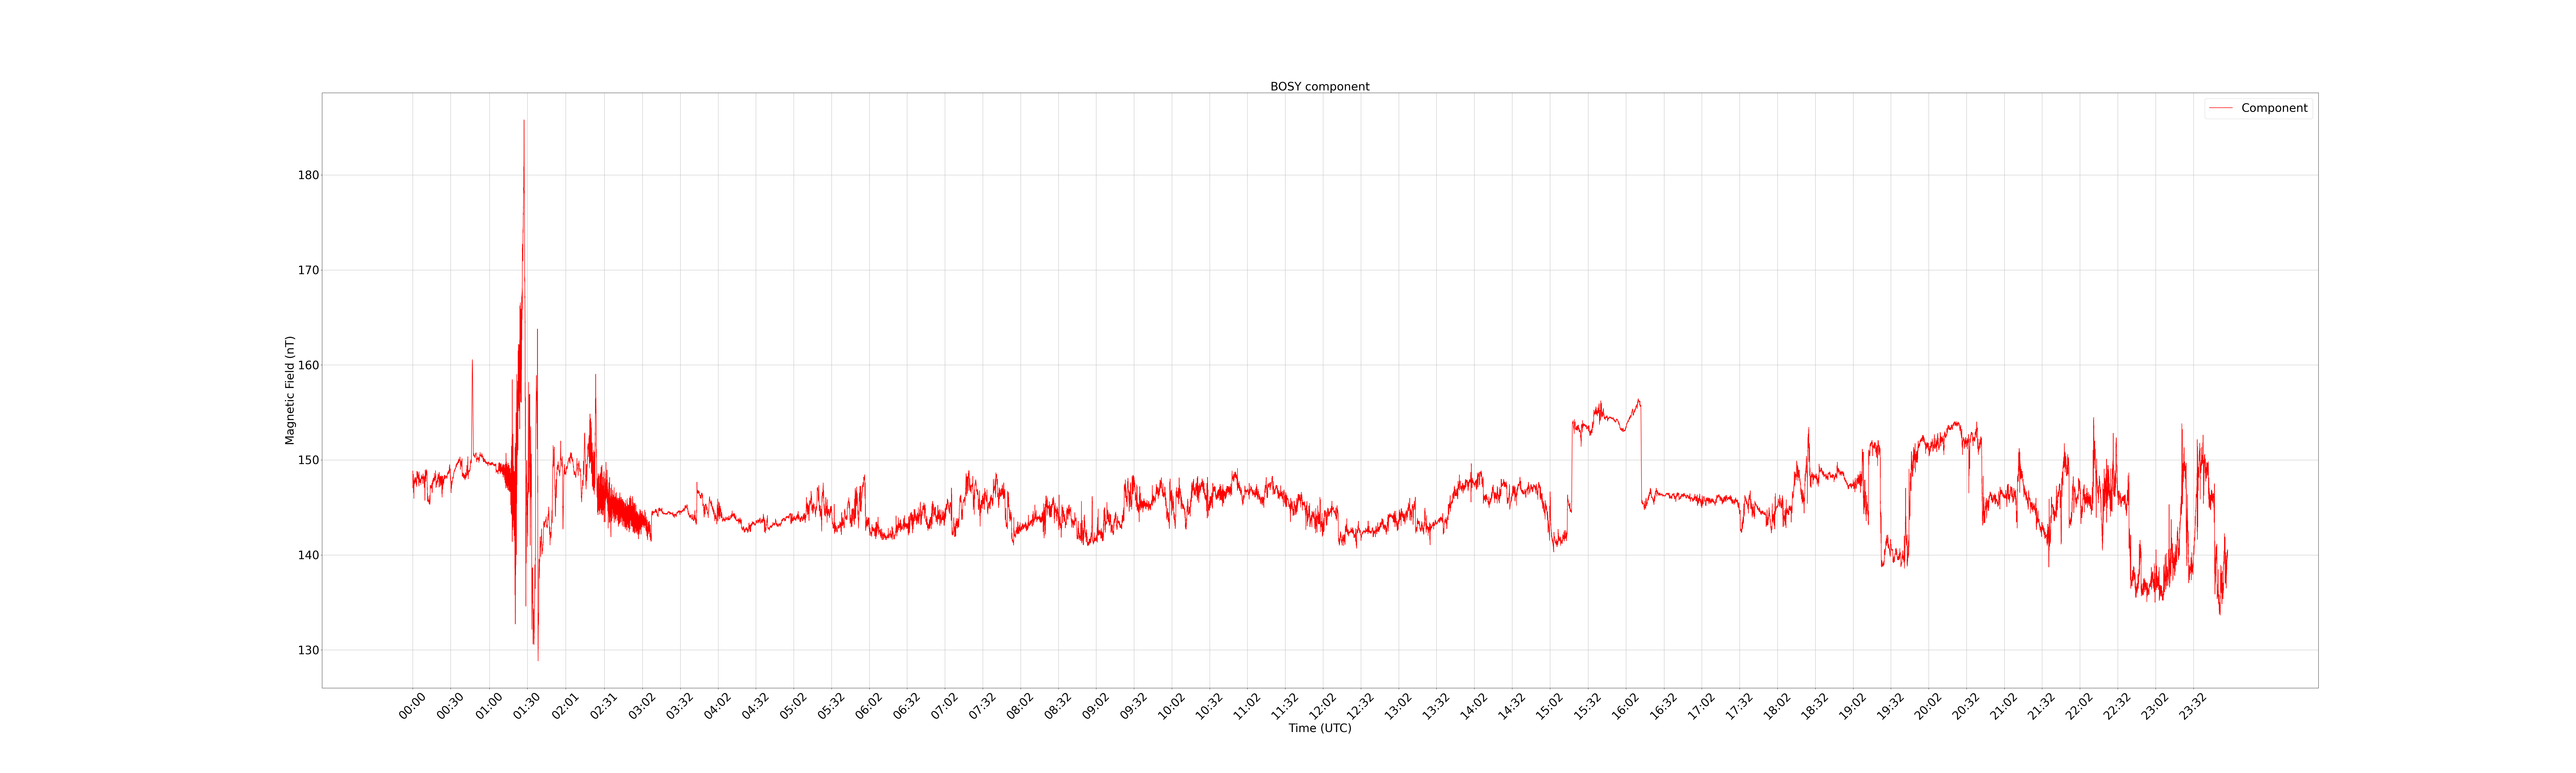
\includegraphics[width=1\linewidth]{../data/assets/BOSY.png}
                \caption{Gráfica de componente BOSY original.}
                \label{fig:bosy-original}
            \end{figure}

            \begin{figure}[!ht]
                \centering
                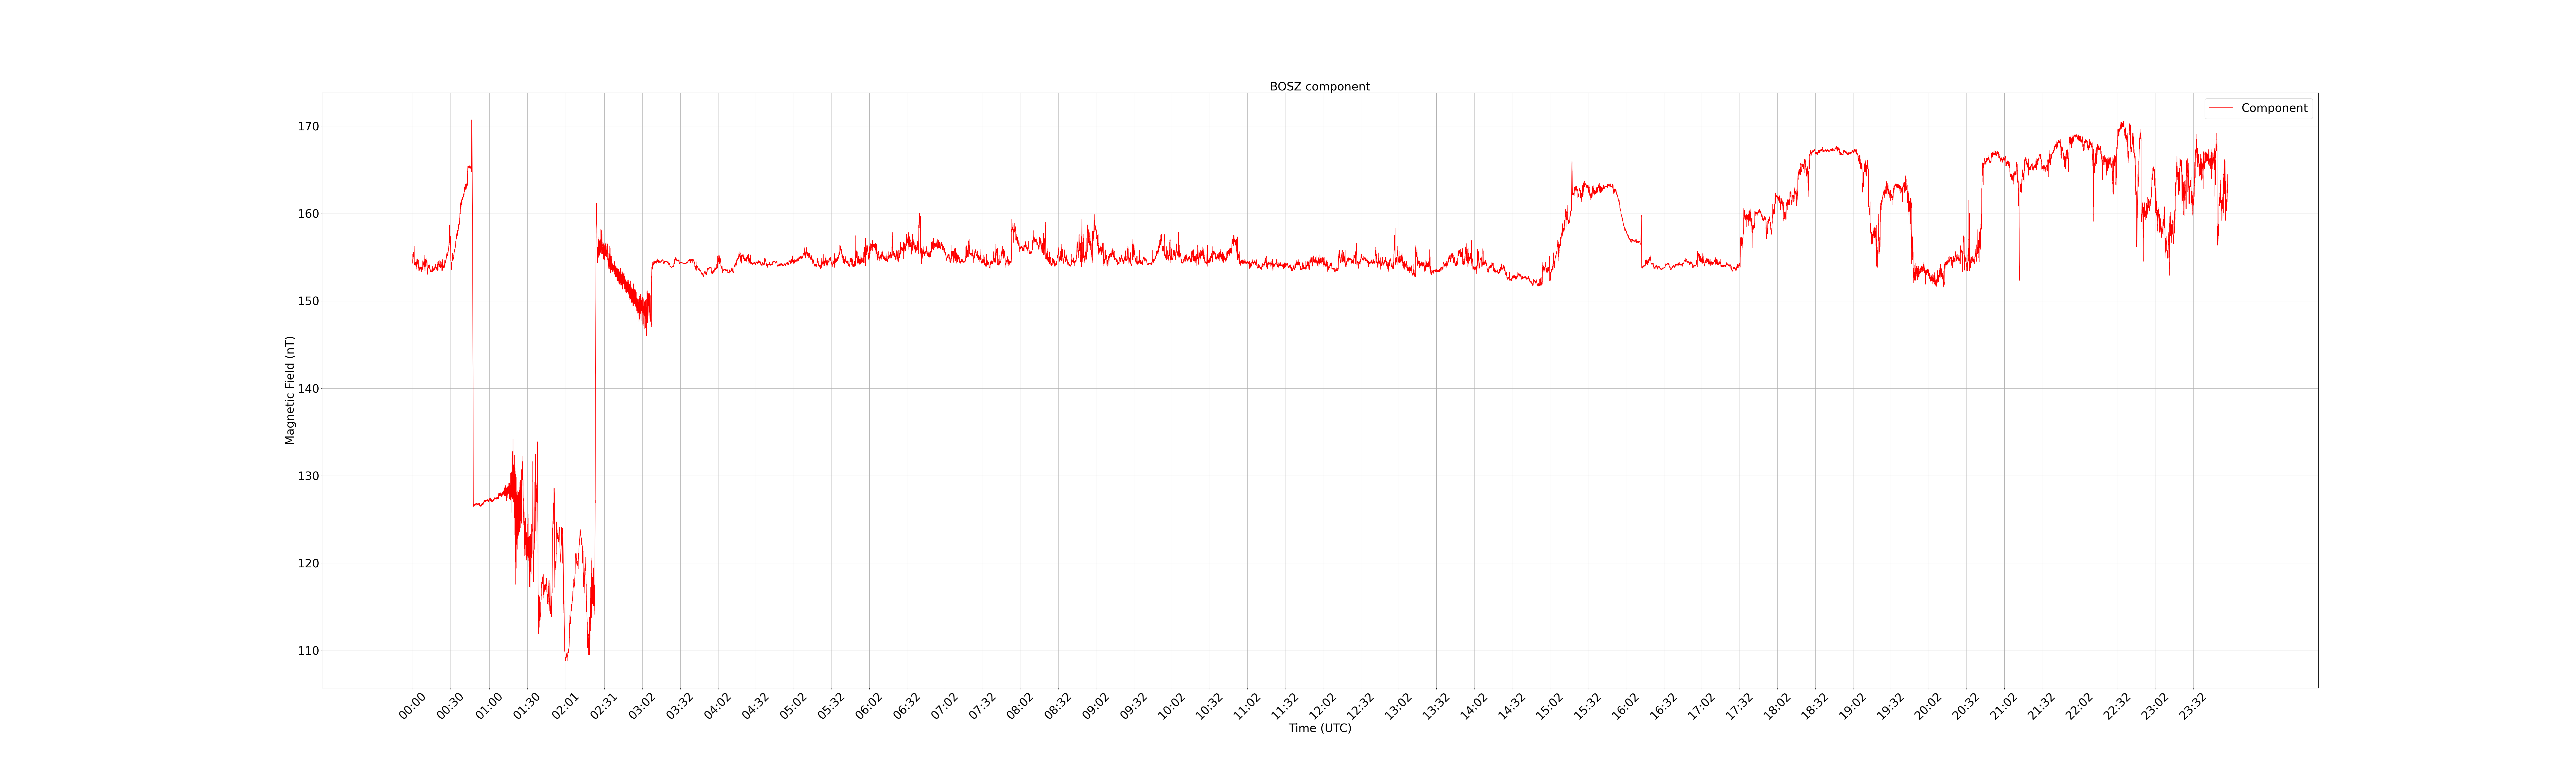
\includegraphics[width=1\linewidth]{../data/assets/BOSZ.png}
                \caption{Gráfica de componente BOSZ original.}
                \label{fig:bosz-original}
            \end{figure}

            Los 3 componentes, tal como se describe en capítulos anteriores, involucra mucho ruido de altas frecuencias en comparación con el comportamiento del campo magnético de Venus.

            Sin embargo, son evidentes las tendencias de cambio principales que se encuentran en un rango muy bajo de frecuencias.

        \subsection{Procesamiento de señales}
            Para comprender mejor las frecuencias que conforman la señal registrada por los sensores BOS, se procesaron las siguientes transformadas discretas de Fourier.

            \begin{figure}[!ht]
                \centering
                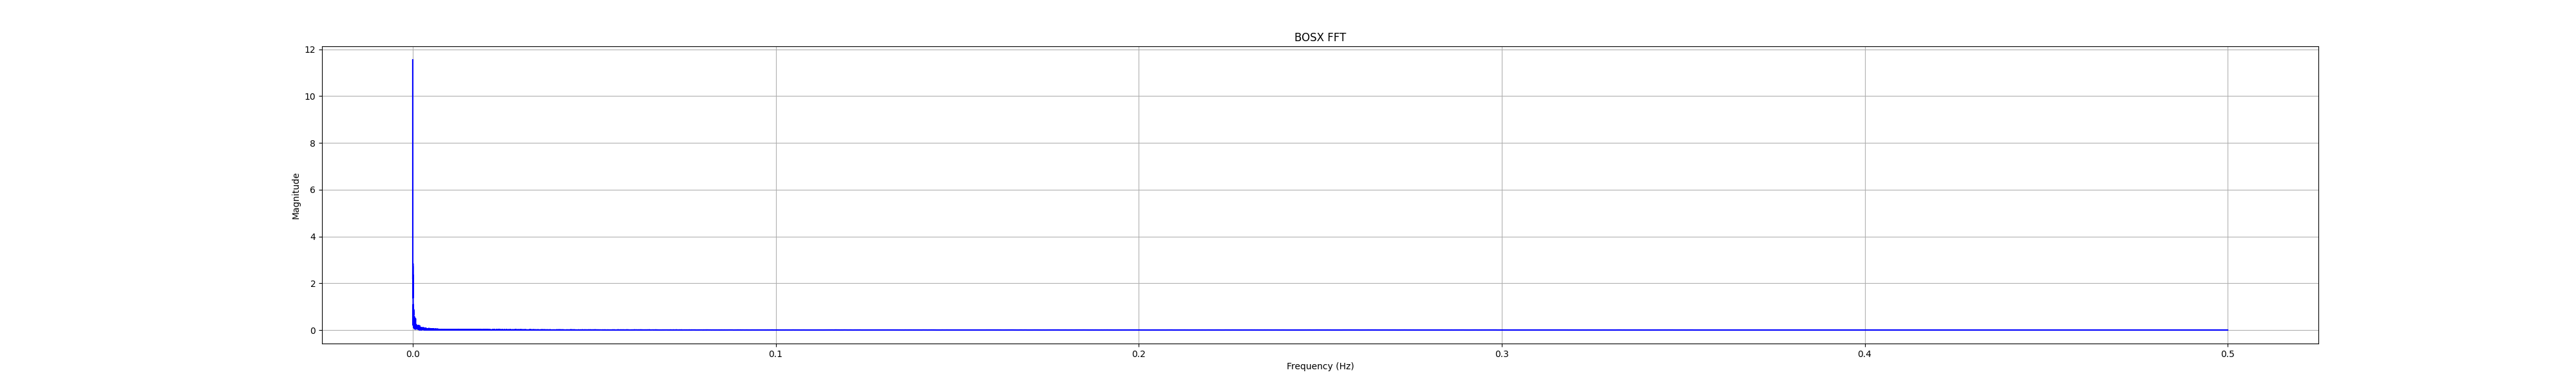
\includegraphics[width=1\linewidth]{../data/assets/frequency_spectrum/BOSX_FFT.png}
                \caption{Gráfica completa de frecuencias para componente BOSX.}
                \label{fig:fft-bosx-complete}
            \end{figure}

            \begin{figure}[!ht]
                \centering
                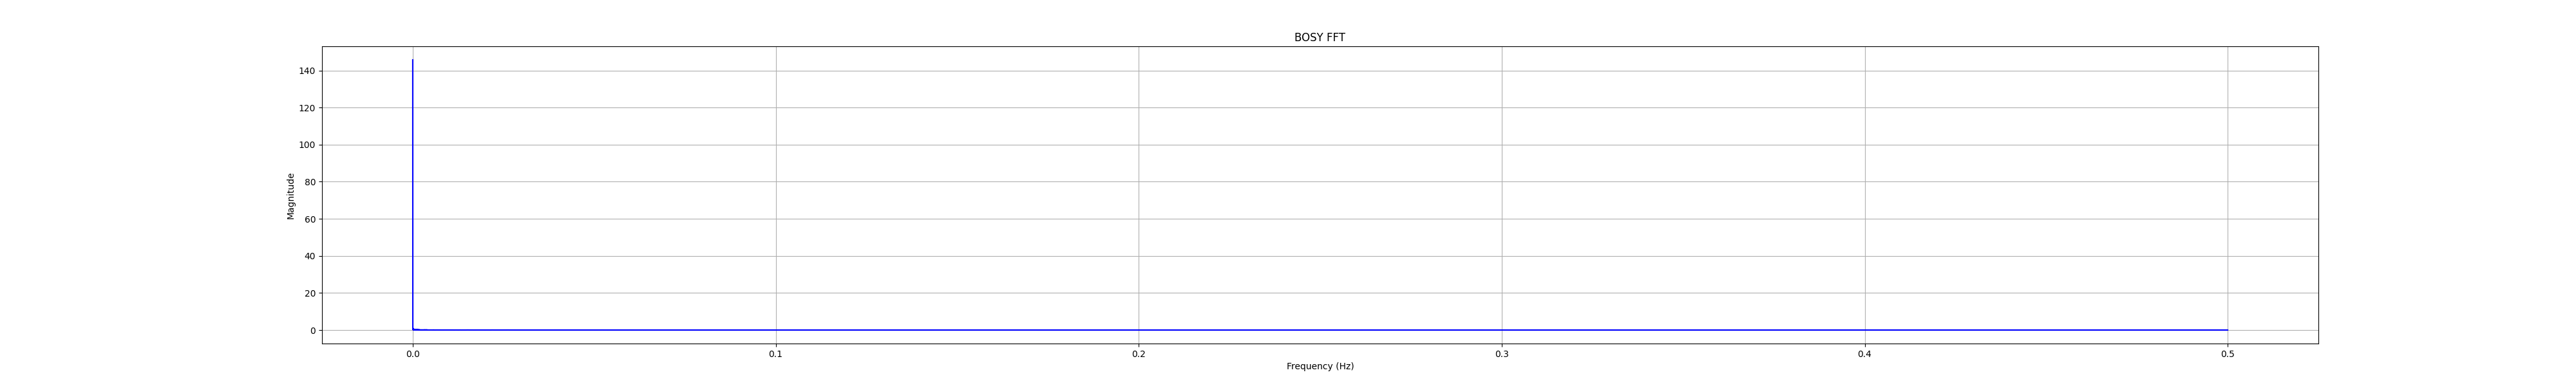
\includegraphics[width=1\linewidth]{../data/assets/frequency_spectrum/BOSY_FFT.png}
                \caption{Gráfica completa de frecuencias para componente BOSY.}
                \label{fig:fft-bosy-complete}
            \end{figure}

            \begin{figure}[!ht]
                \centering
                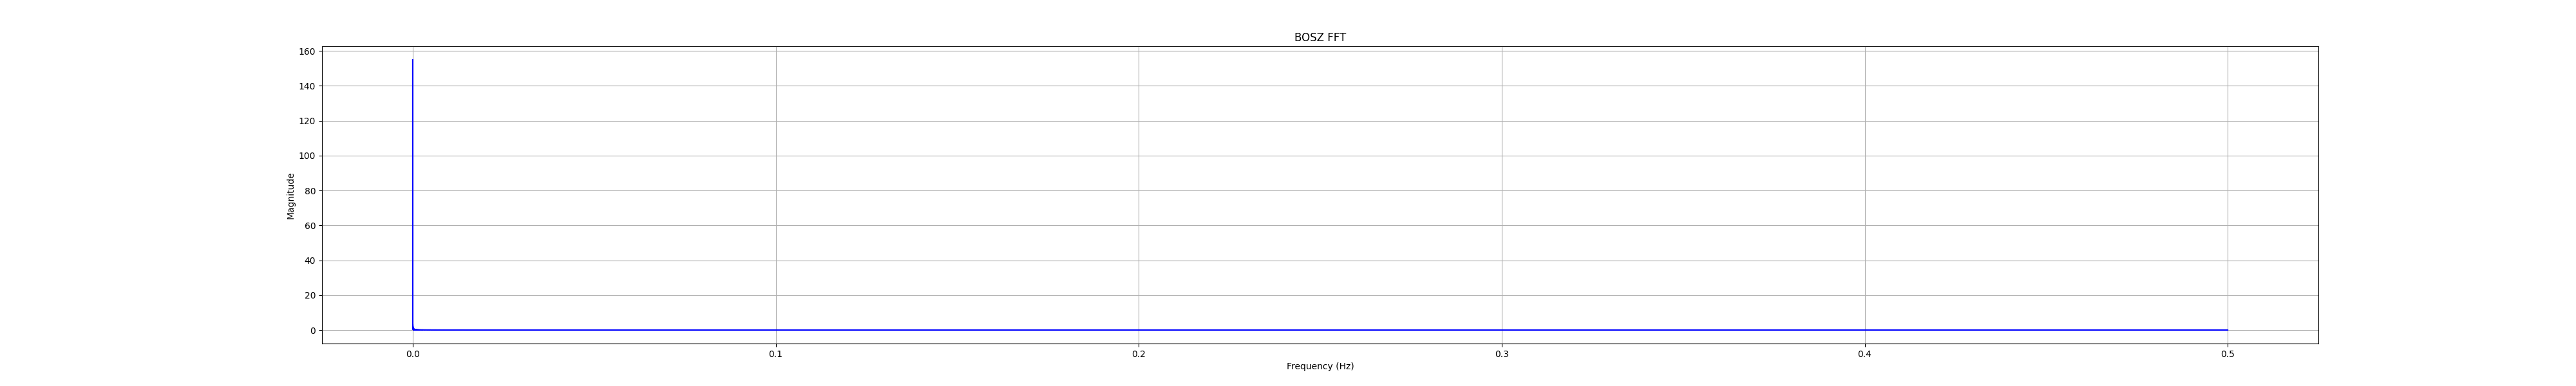
\includegraphics[width=1\linewidth]{../data/assets/frequency_spectrum/BOSZ_FFT.png}
                \caption{Gráfica completa de frecuencias para componente BOSZ.}
                \label{fig:fft-bosz-complete}
            \end{figure}

            En las tres transformaciones resultantes se puede observar que frecuencias muy cercanas a 0 predominan en la señal de cada componente.

            Para obtener un análisis más detallado, se dibujaron los primeros 150 componentes de las frecuencias de cada señal, mismas que se visualizan en las ilustraciones 7, 8 y 9 para los componentes BOSX, BOSY y BOSZ correspondientemente.

            \begin{figure}[!ht]
                \centering
                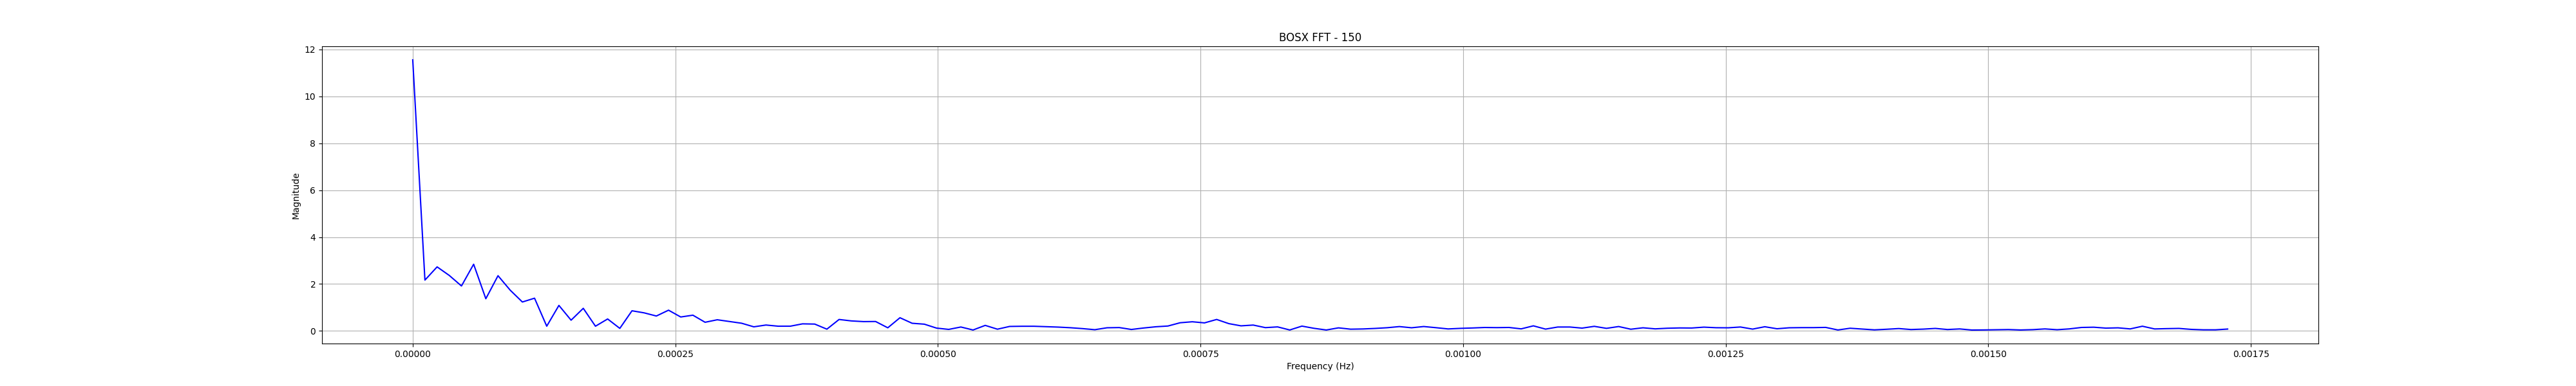
\includegraphics[width=1\linewidth]{../data/assets/frequency_spectrum/BOSX_FFT_150.png}
                \caption{Gráfica de frecuencias para componente BOSX con los primeros 150 elementos.}
                \label{fig:fft-bosx-partial}
            \end{figure}

            \newpage
            \begin{figure}[!ht]
                \centering
                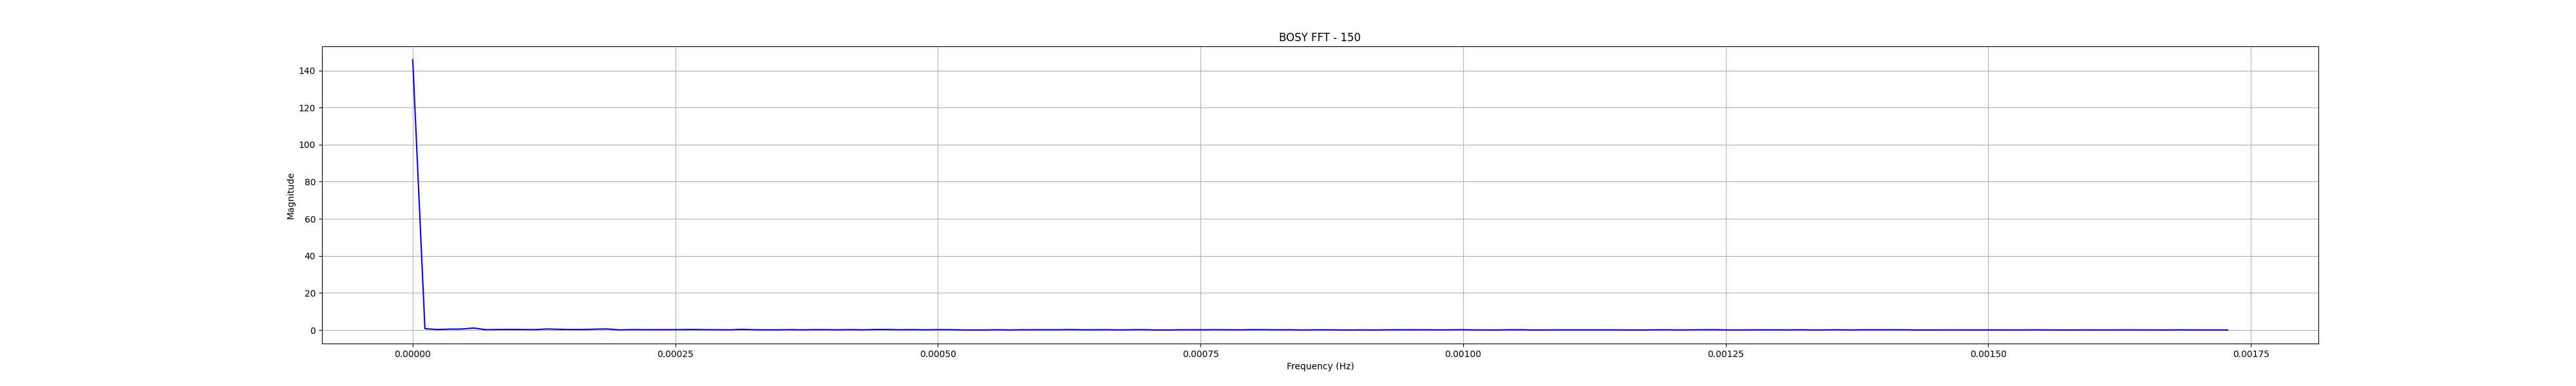
\includegraphics[width=1\linewidth]{../data/assets/frequency_spectrum/BOSY_FFT_150.png}
                \caption{Gráfica de frecuencias para componente BOSY con los primeros 150 elementos.}
                \label{fig:fft-bosy-partial}
            \end{figure}

            \begin{figure}[!ht]
                \centering
                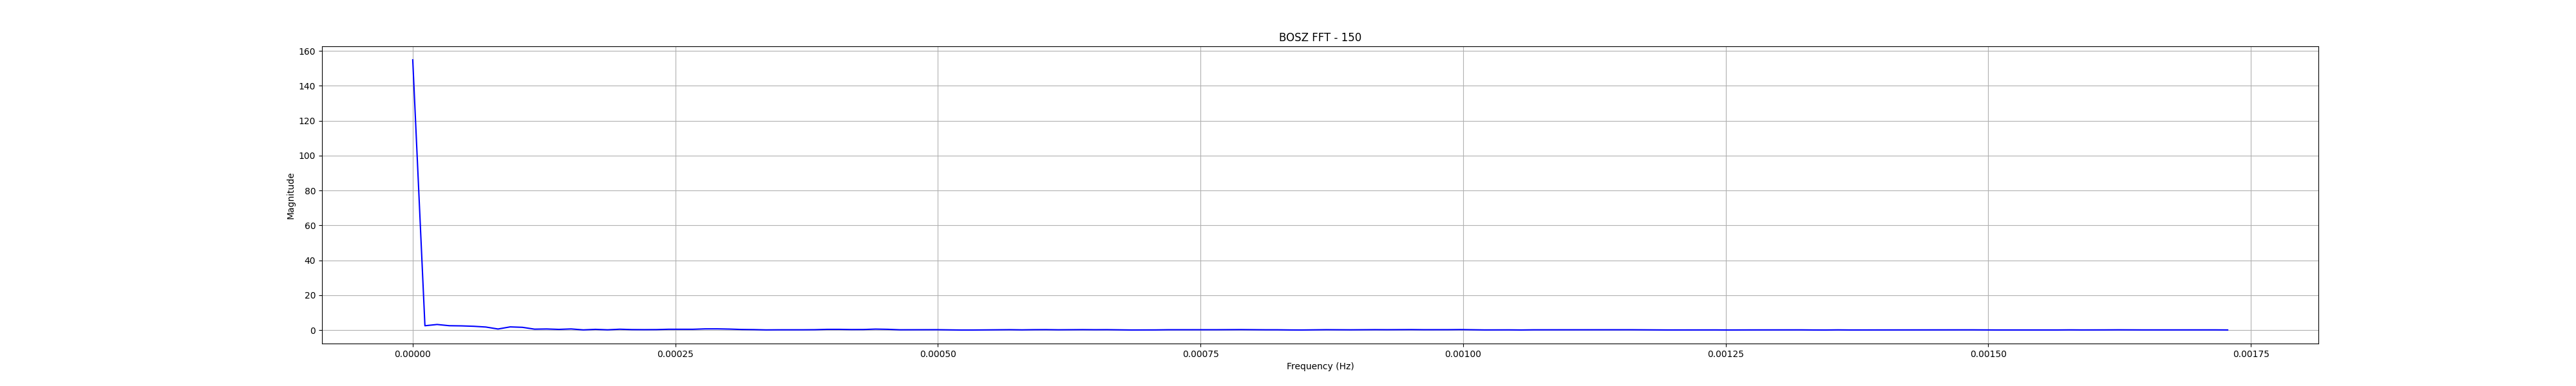
\includegraphics[width=1\linewidth]{../data/assets/frequency_spectrum/BOSZ_FFT_150.png}
                \caption{Gráfica de frecuencias para componente BOSZ con los primeros 150 elementos.}
                \label{fig:fft-bosz-partial}
            \end{figure}

            En los componentes BOSY y BOSZ, la señal le da más relevancia a frecuencias cercanas a 0 y no mayores a $2.5\cdot 10^{-4} Hz$. Por otro lado, la señal de BOSX presenta un rango más amplio de frecuencias con un coeficiente mayor a 0. Esto significa que la señal BOSX tiene una contaminación considerable.

            Para mantener los componentes de frecuencia congruentes entre las 3 señales y no perder los mínimos y máximos globales de la señal, se optó por eliminar las frecuencias superiores a $5\cdot 10^{-5}Hz$. Los resultados de este filtro se ven en las figuras 10, 11 y 12.

            \begin{figure}[!ht]
                \centering
                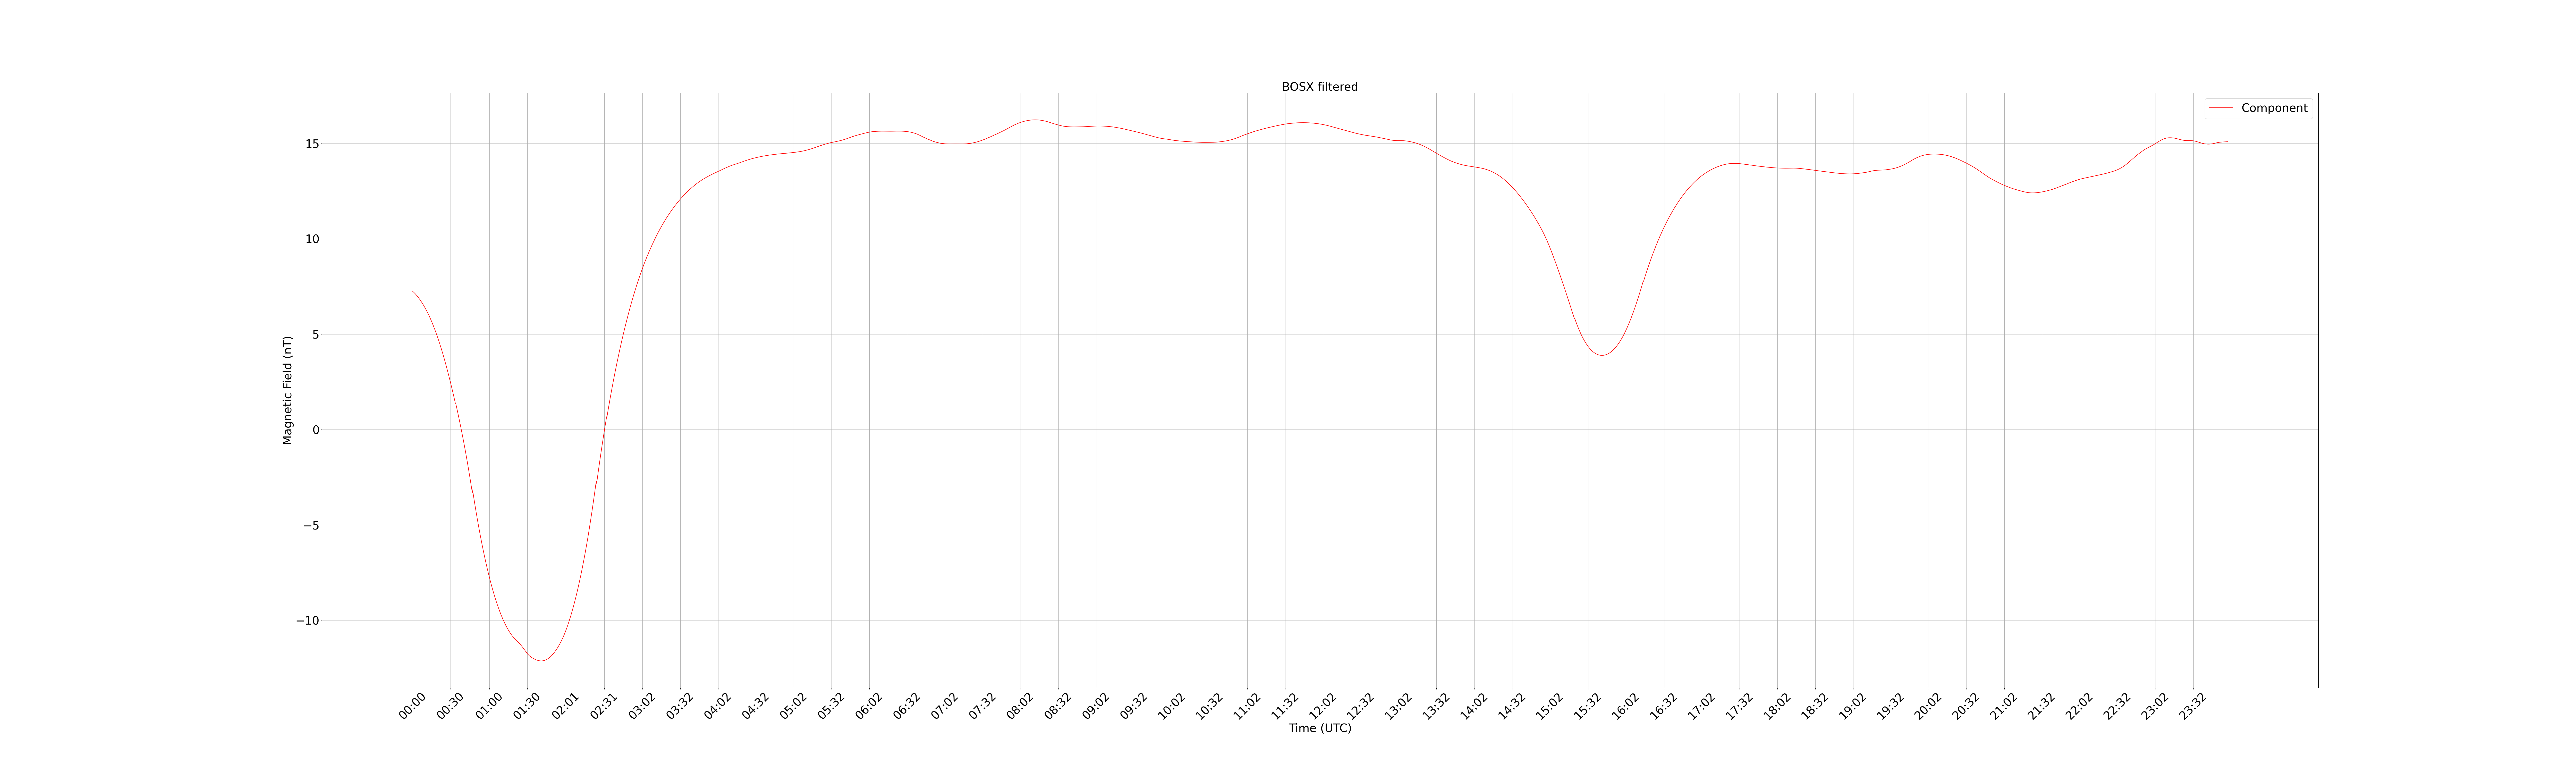
\includegraphics[width=1\linewidth]{../data/assets/filtered/BOSX_high_frequency_filter.png}
                \caption{Gráfica de señal BOSX tras aplicar filtro pasa-bajas.}
                \label{fig:bosx-hff}
            \end{figure}
	
	        \newpage
            \begin{figure}[!ht]
                \centering
                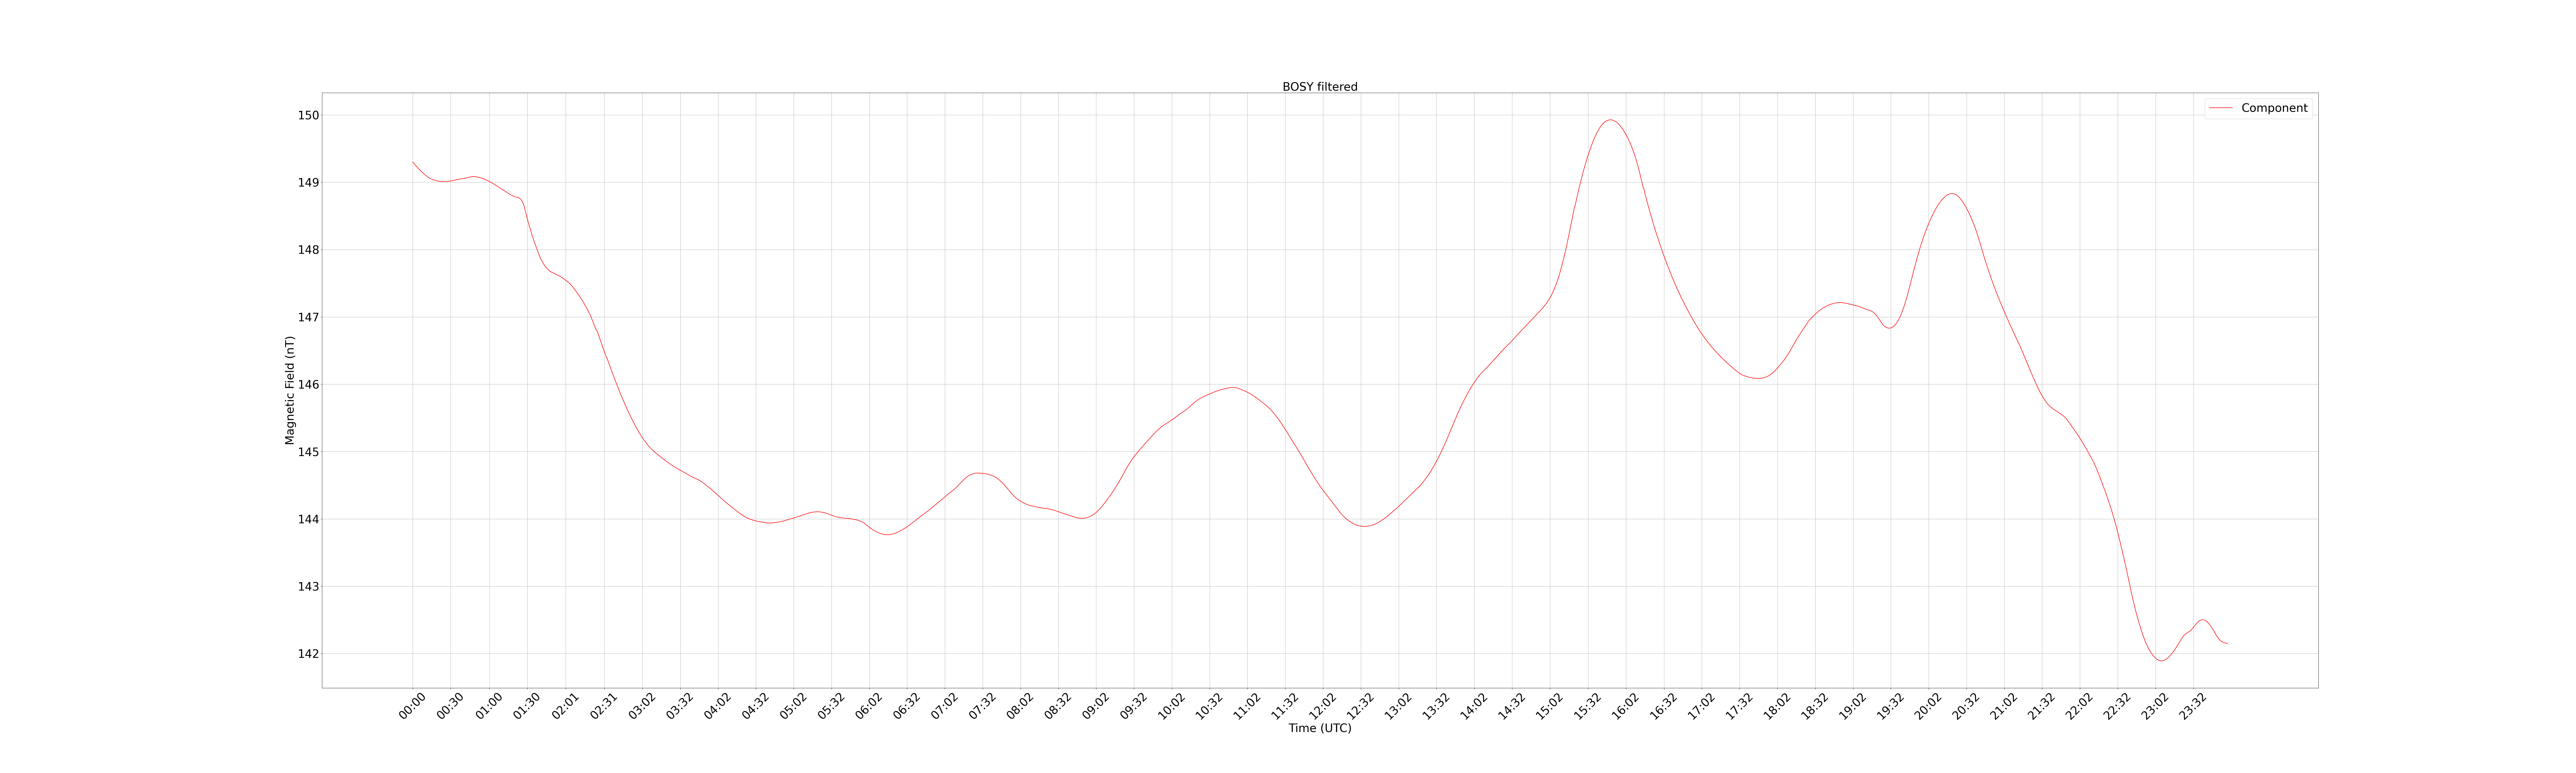
\includegraphics[width=1\linewidth]{../data/assets/filtered/BOSY_high_frequency_filter.png}
                \caption{Gráfica de señal BOSY tras aplicar filtro pasa-bajas.}
                \label{fig:bosy-hff}
            \end{figure}

            \begin{figure}[!ht]
                \centering
                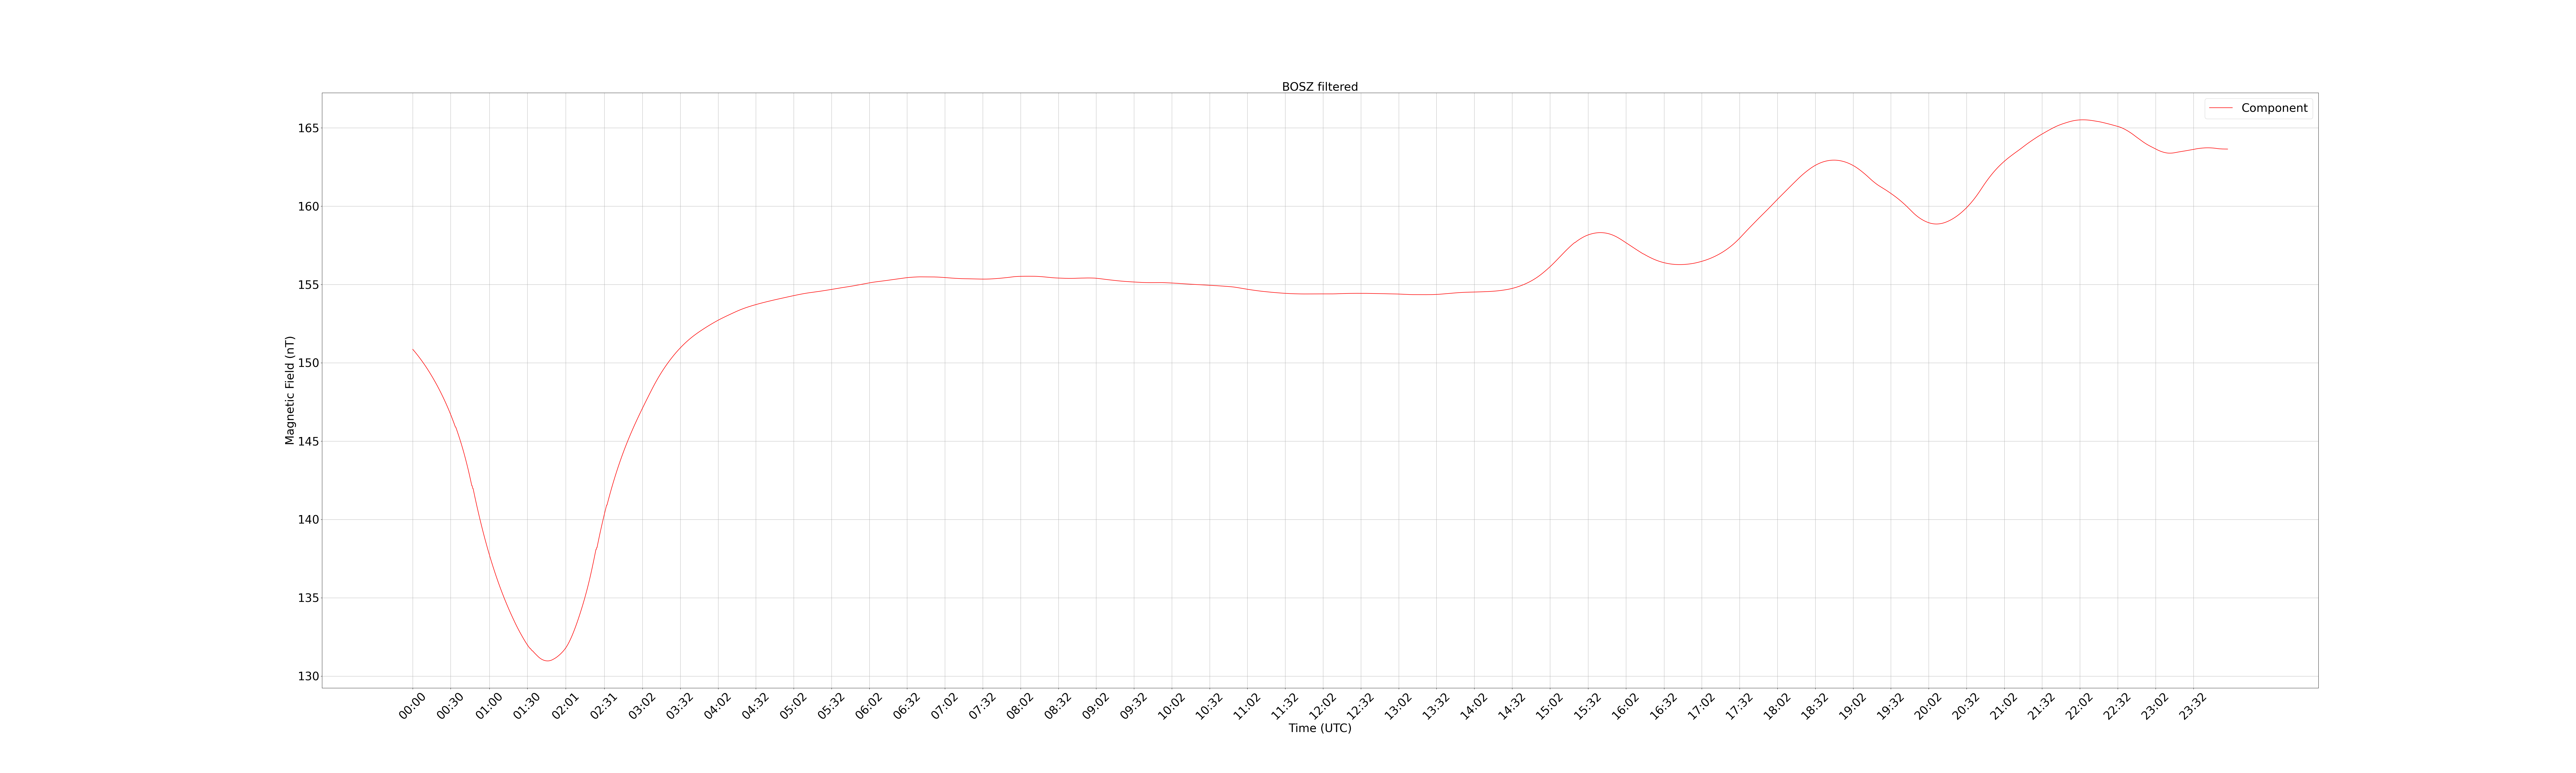
\includegraphics[width=1\linewidth]{../data/assets/filtered/BOSZ_high_frequency_filter.png}
                \caption{Gráfica de señal BOSZ tras aplicar filtro pasa-bajas.}
                \label{fig:bosz-hff}
            \end{figure}

            Estas señales filtradas, por sí solas, muestran congruencia con la señal esperada. Las transformaciones de Fourier de las tres señales se ilustran a continuación.

            \begin{figure}[!ht]
               \centering
                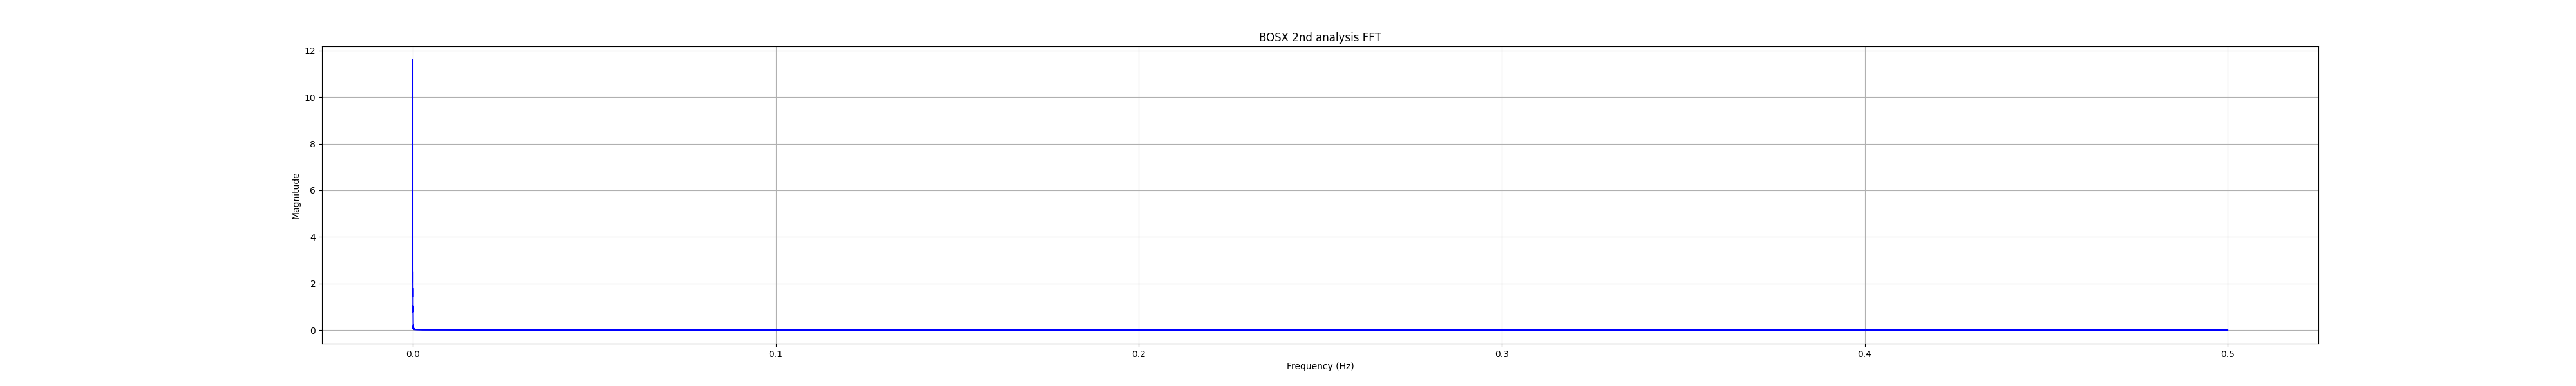
\includegraphics[width=1\linewidth]{../data/assets/frequency_spectrum/BOSX_FFT_hff.png}
                \caption{Gráfica completa de frecuencias para componente BOSX.}
                \label{fig:fft-hff-bosx-complete}
            \end{figure}

            \begin{figure}[!ht]
                \centering
                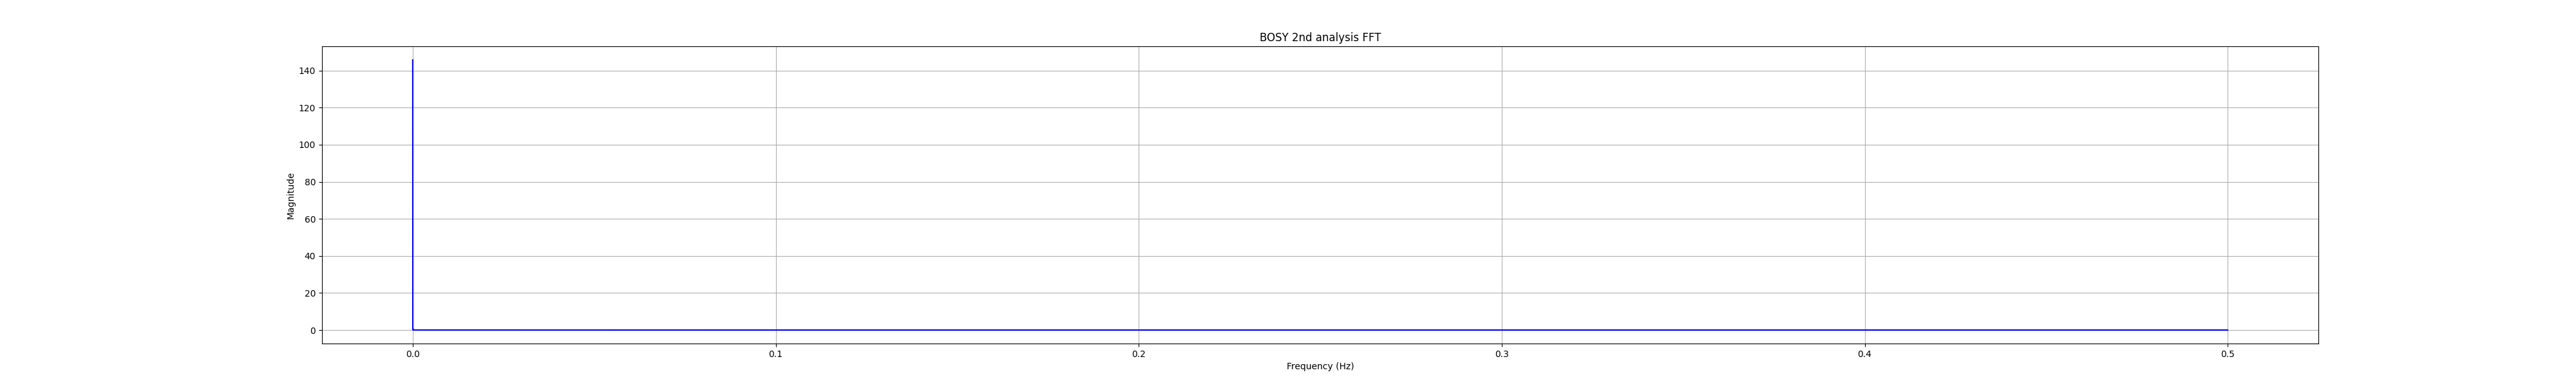
\includegraphics[width=1\linewidth]{../data/assets/frequency_spectrum/BOSY_FFT_hff.png}
                \caption{Gráfica completa de frecuencias para componente BOSY.}
                \label{fig:fft-hff-bosy-complete}
            \end{figure}
	
	  \newpage
            \begin{figure}[!ht]
                \centering
                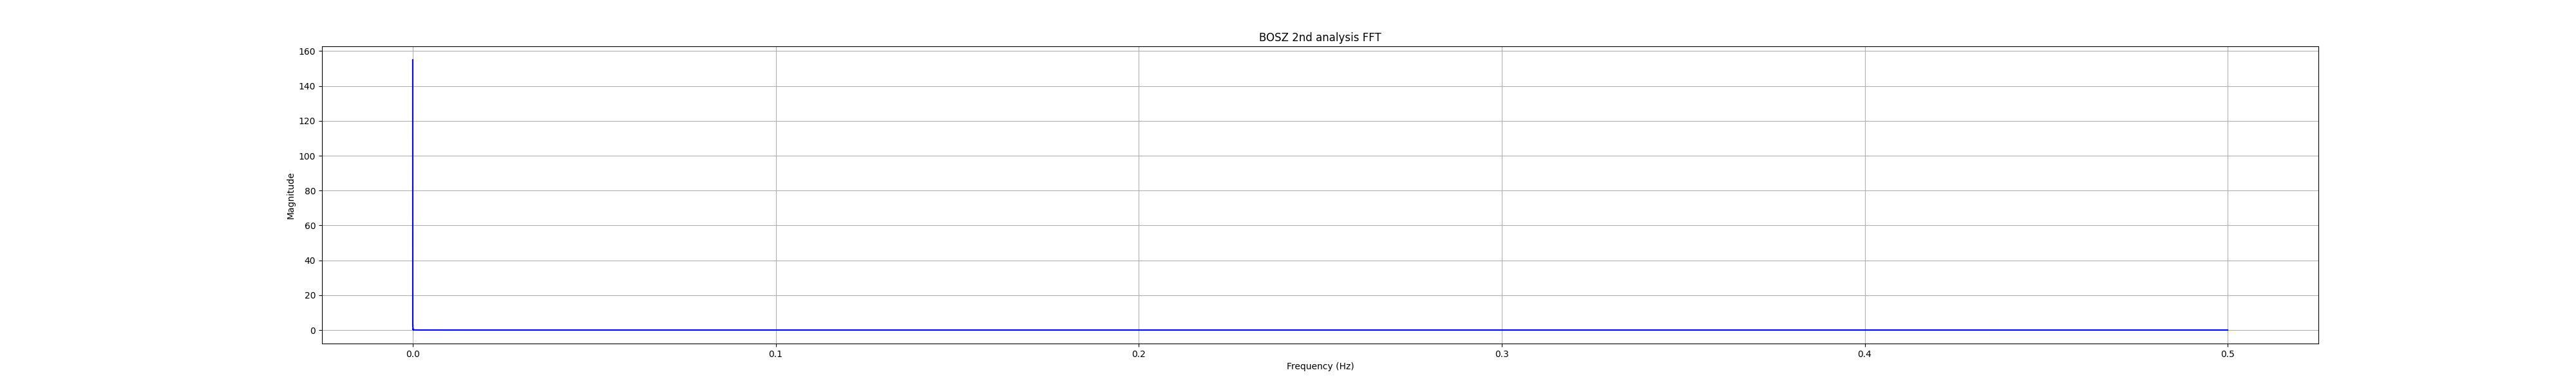
\includegraphics[width=1\linewidth]{../data/assets/frequency_spectrum/BOSZ_FFT_hff.png}
                \caption{Gráfica completa de frecuencias para componente BOSZ.}
                \label{fig:fft-hff-bosz-complete}
            \end{figure}

	  Para un mejor análisis, se dibujaron las gráficas de los primeros 25 componentes de frecuencia de las señales.
	  
	  \begin{figure}[!ht]
               \centering
                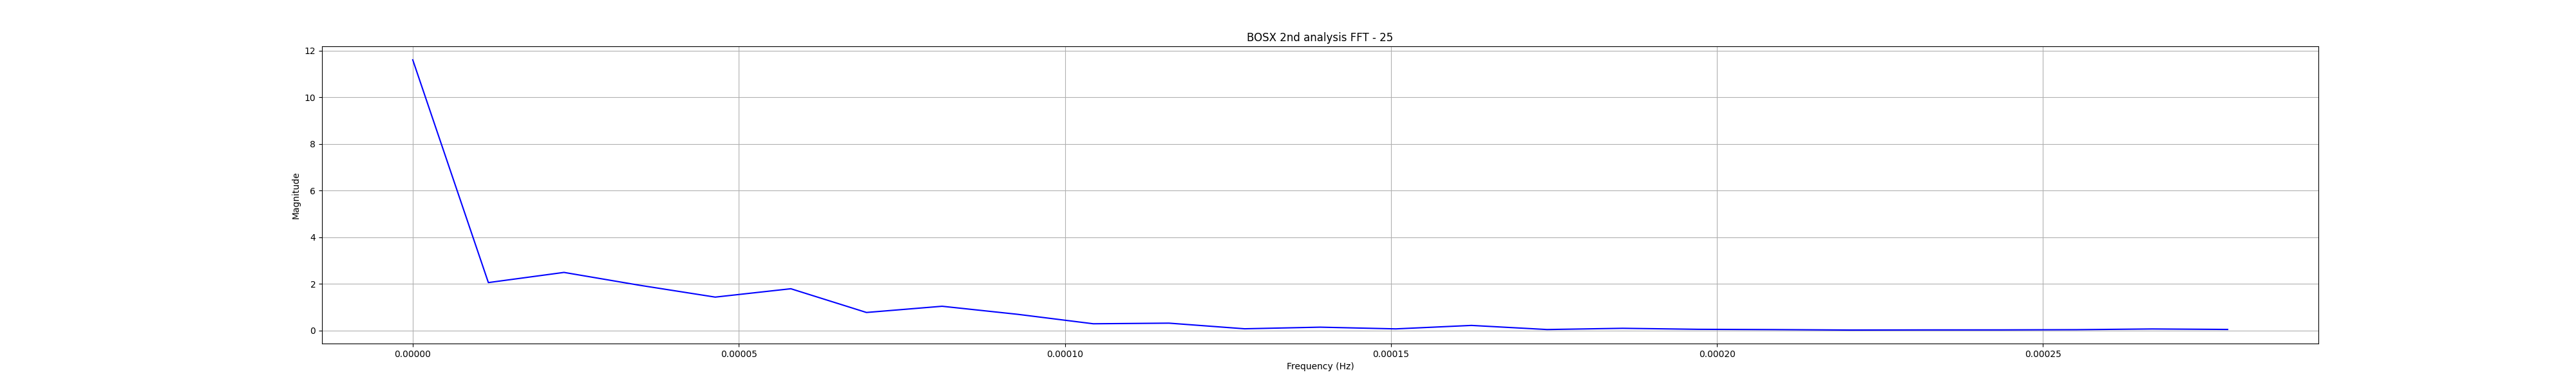
\includegraphics[width=1\linewidth]{../data/assets/frequency_spectrum/BOSX_FFT_hff_25.png}
                \caption{Gráfica parcial de frecuencias para componente BOSX.}
                \label{fig:fft-hff-bosx-partial}
            \end{figure}

	  \begin{figure}[!ht]
               \centering
                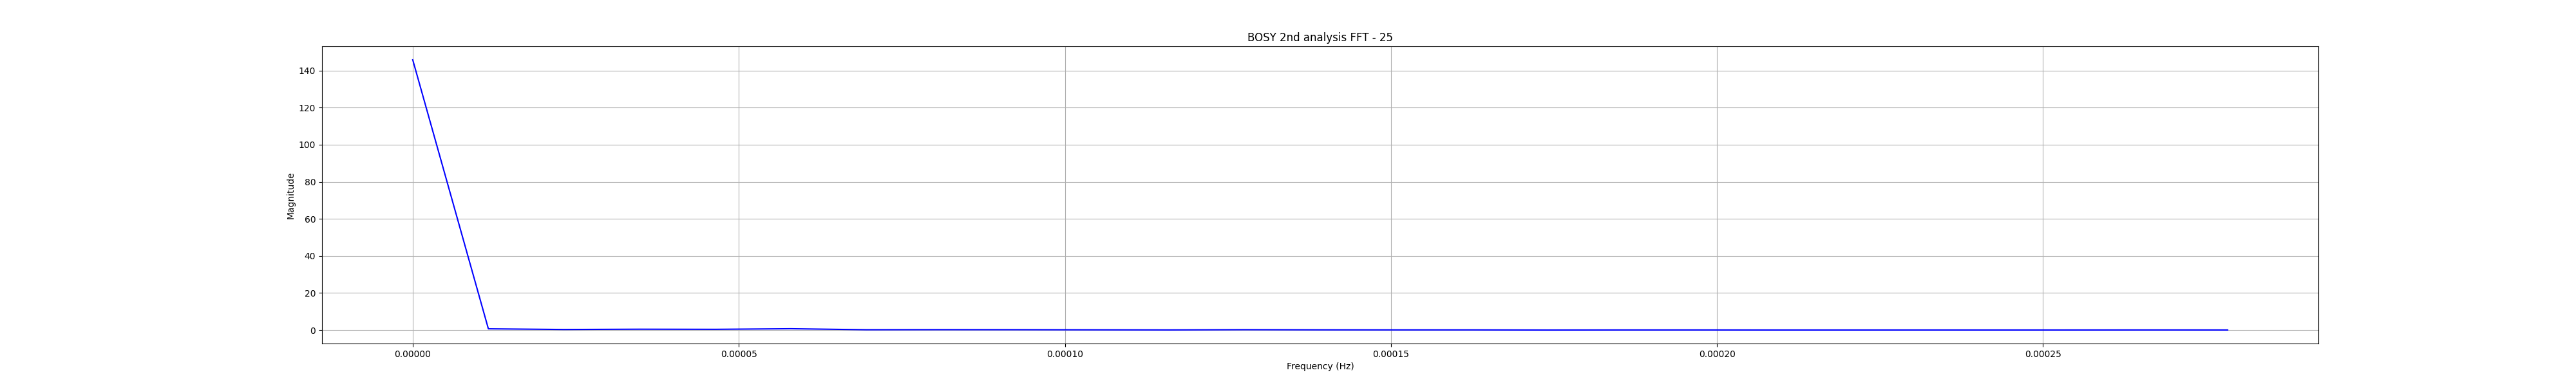
\includegraphics[width=1\linewidth]{../data/assets/frequency_spectrum/BOSY_FFT_hff_25.png}
                \caption{Gráfica parcial de frecuencias para componente BOSY.}
                \label{fig:fft-hff-bosy-partial}
            \end{figure}

	  \begin{figure}[!ht]
               \centering
                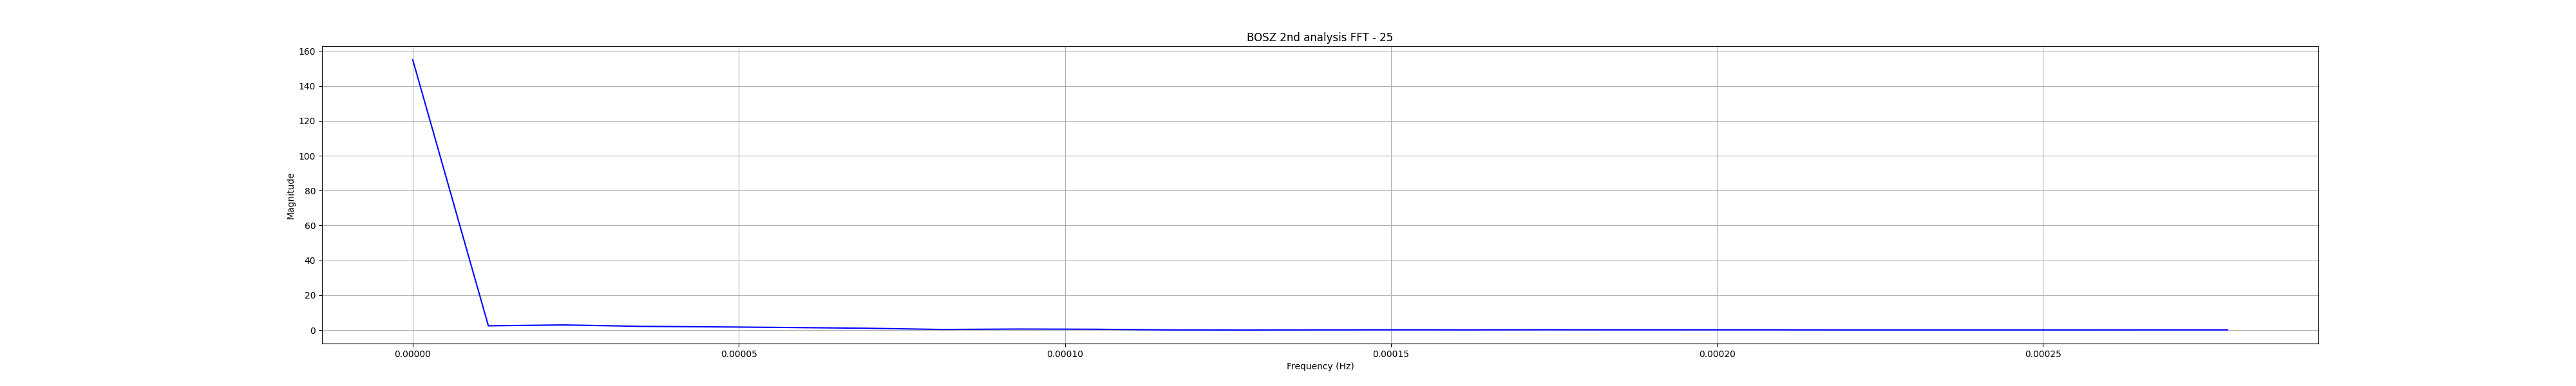
\includegraphics[width=1\linewidth]{../data/assets/frequency_spectrum/BOSZ_FFT_hff_25.png}
                \caption{Gráfica parcial de frecuencias para componente BOSZ.}
                \label{fig:fft-hff-bosz-partial}
            \end{figure}

	  Tras experimentar con la aplicación de otros filtros, se llegó a la conclusión de que cualquier intento de eliminar el resto de frecuencias de ruido impacta gravemente en la captura del fenómeno estudiado.

        \subsection{Cálculo del módulo total}
	  Posterior a la limpieza de la señal, se procede a calcular la magnitud absoluta de la señal a lo largo del tiempo. La señal resultante (BOST filtrada) se ilustra en la siguiente figura.

	  \begin{figure}[!ht]
               \centering
                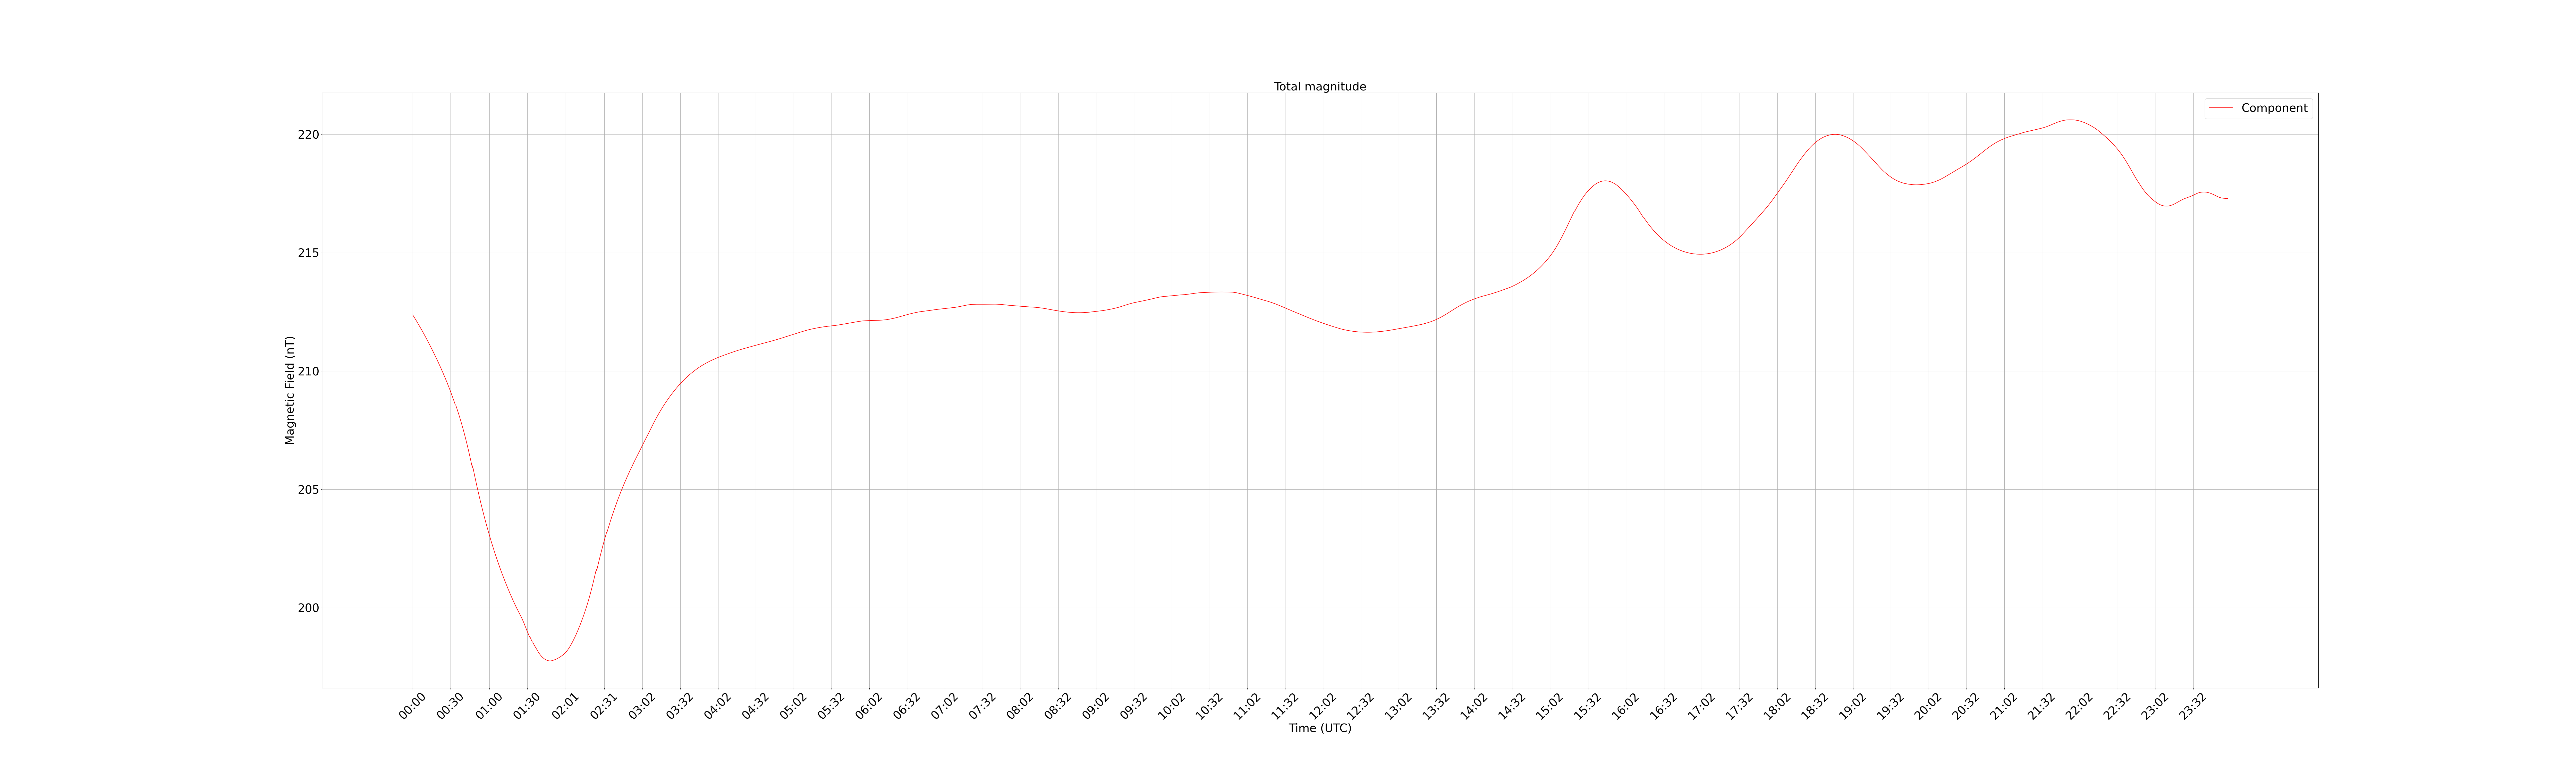
\includegraphics[width=1\linewidth]{../data/assets/filtered/BOST_filtering_result.png}
                \caption{Gráfica de señal BOST filtrada.}
                \label{fig:bost-filtered}
            \end{figure}
	  \newpage

        \subsection{Comparación con BOST de la ESA}
	  Finalmente, para evidenciar el contraste entre la señal original y la procesada, en la figura 20 se dibujan ambas señales.
	  \begin{figure}[!ht]
               \centering
                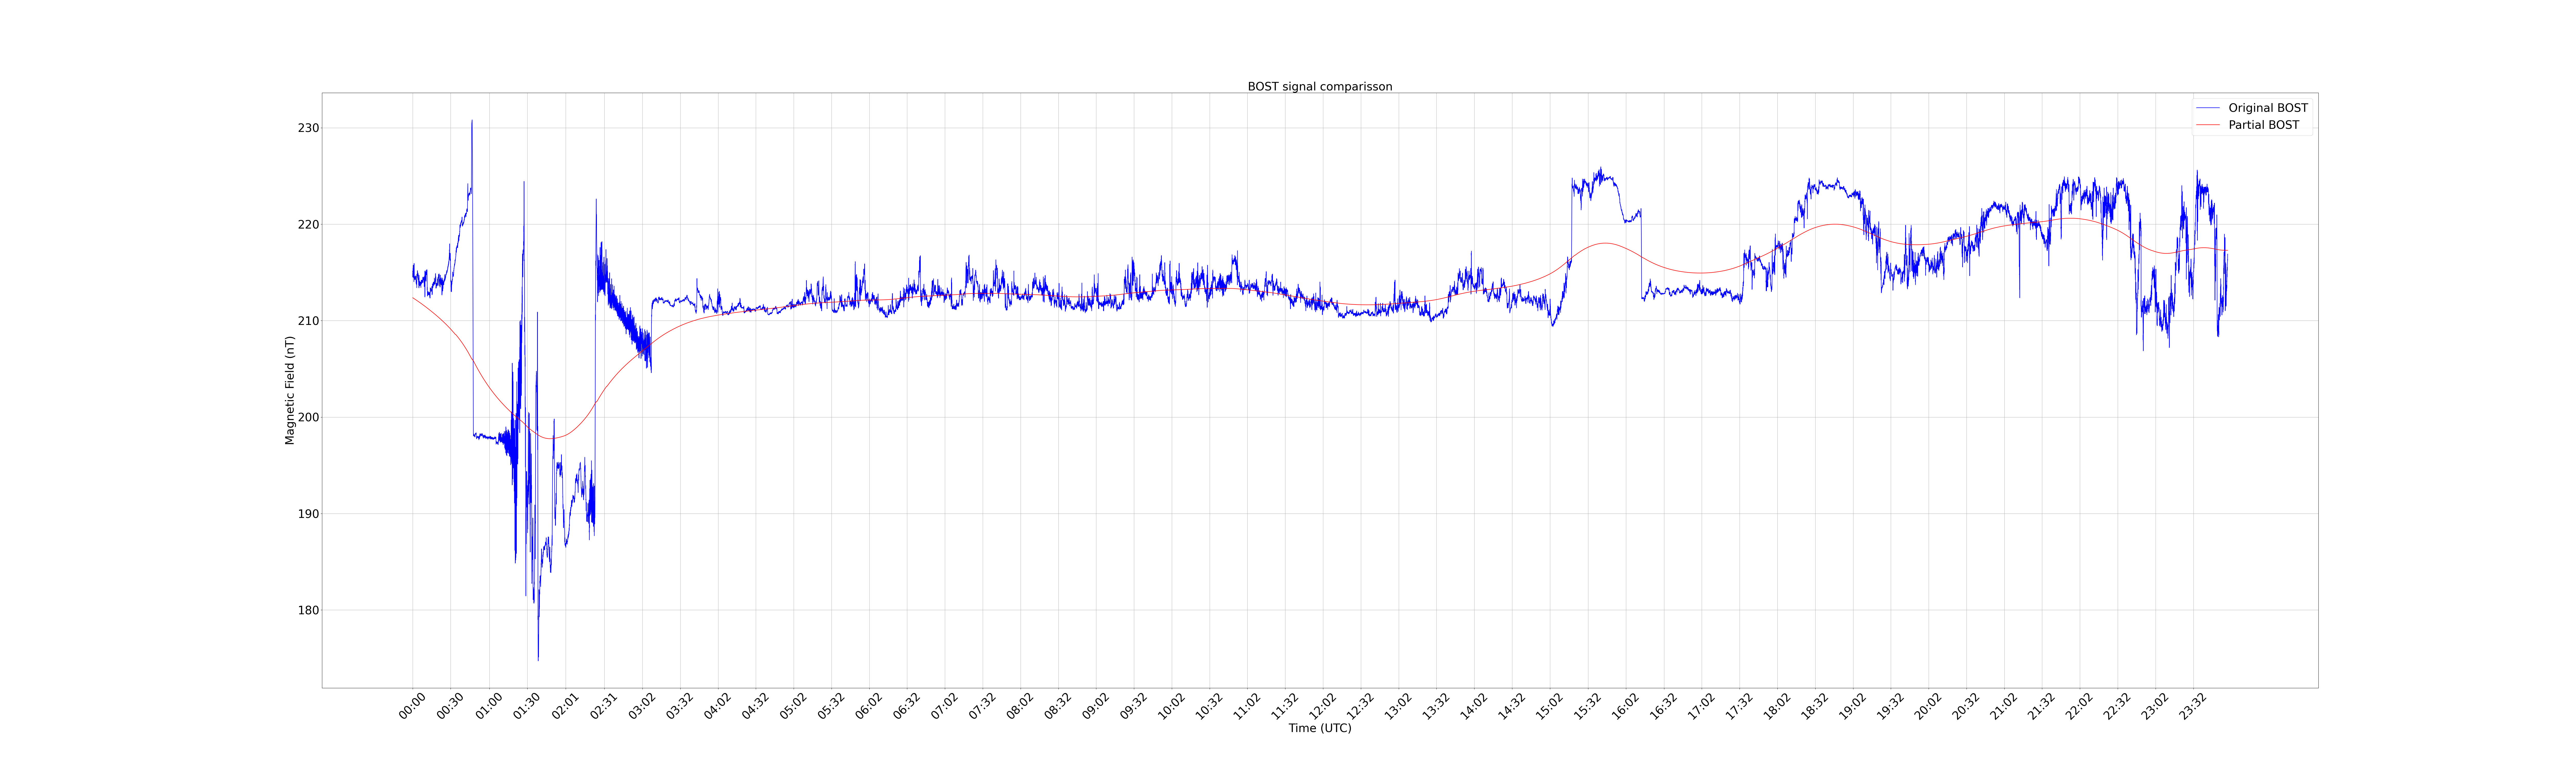
\includegraphics[width=1\linewidth]{../data/assets/BOST_comparisson.png}
                \caption{Gráfica de comparación entre BOST original y BOST filtrada.}
                \label{fig:bost-comparisson}
            \end{figure}
    \section{Conclusiones}
	  \subsection{Interpretación de la señal resultante}
	  	  De acuerdo con el contexto anteriormente mencionado, esta señal indica que el campo magnético presente en Venus es uno meramente reactivo ante la actividad solar, puesto que, al encontrarse en la cara opuesta al sol de Venus, el campo magnético desciende a valores muy bajos, evidenciando que el planeta no genera su propio campo magnético ocasionado por algún otro fenómeno interno que no involucre la ionósfera. Por lo tanto, Venus no tiene un campo magnético propio.
	  \subsection{Aplicación de filtros}
	  	  Las herramientas estudiadas en el semestre permitieron analizar y filtrar aceptablemente la señal que refleja el comportamiento de un fenómeno real. Esto, en consecuencia, demuestra que las herramientas estudiadas permiten el diseño de métodos de tratamiento y adquisición de señales discretas muestreadas por instrumentos digitales.

    \begin{thebibliography}{10}

        \bibitem{zhan2006}
T. L. Zhang et al., “Magnetic field investigation of the Venus plasma environment: Expected new results from Venus Express,” Planetary and Space Science, vol. 54, no. 13–14, pp. 1336–1343, Noviembre 2006. [En línea]. Disponible en: \url{https://www.sciencedirect.com/science/article/abs/pii/S0032063306001607?via%3Dihub}. Último acceso: 15 de junio de 2025.
        \bibitem{esa}
 European Space Agency, \textit{“Venus Express overview,”} ESA Science \& Exploration, 21 de junio de 2006.[En línea]. Disponible en: \url{https://www.esa.int/Science_Exploration/Space_Science/Venus_Express_overview}. Último acceso: 14 de junio de 2025.
        \bibitem{nasa2025}
NASA, \textit{“Venus Facts,”} NASA Science, 21 de abril de 2025. [En línea]. Disponible en: \url{https://science.nasa.gov/venus/venus-facts/}. Último acceso: 14 de junio de 2025.
        \bibitem{solarorbiter2021}
 NASA, \textit{“Solar Orbiter revela detalles sobre el entorno magnético de Venus,”} NASA Ciencia, 3 de mayo de 2021. [En línea]. Disponible en: \url{https://ciencia.nasa.gov/sistema-solar/solar-orbiter-campo-magnetico-venus/}. Último acceso: 14 de junio de 2025.
        \bibitem{patzold2007}
 M. Pätzold et al., \textit{"The structure of Venus’ middle atmosphere and ionosphere,"} Nature, vol. 450, pp. 657–660, Nov. 2007. Disponible en: \url{https://www.nature.com/articles/nature06239#citeas}. Último acceso: 14 de junio de 2025.
        \bibitem{esaorbita}
 European Space Agency (ESA), \textit{"Operational orbit,"} Venus Express, 17 de Octubre de 2005. [En línea]. Disponible en: \url{https://sci.esa.int/web/venus-express/-/37357-operational-orbit}. [Último acceso : 17 de junio de 2025].
        \bibitem{esa2}
 T. L. Zhang et al., \textit{"MAG: The Fluxgate Magnetometer of Venus Express"}. European Space Agency (ESA), Scientific Instrument Documentation, ESA SP-1295, 2007. [En línea]. Disponible en: \url{https://sci.esa.int/documents/34571/36233/1567256675388-MagWeb.pdf}. Último acceso: 14 de junio de 2025.
        \bibitem{Mc2000}
R. N. Bracewell, \textit{"The Fourier Transform and Its Applications"}, 3rd ed. Boston, MA, USA: McGraw-Hill, 2000.
[En línea]. Disponible en: \url{https://archive.org/details/TheFourierTransformAndItsApplicationsBracewell/page/n3/mode/2up}. Último acceso: 17 de junio de 2025. 
        \bibitem{oppenheim2010}
A. V. Oppenheim and R. W. Schafer, \textit{"Discrete\-Time Signal Processing"}, 3rd ed. Upper Saddle River, NJ, USA: Pearson, 2010. [En línea]. Disponible en : \url{https://file.fouladi.ir/courses/dsp/books/%28Prentice-Hall%20Signal%20Processing%20Series%29%20Alan%20V.%20Oppenheim%2C%20Ronald%20W.%20Schafer-Discrete-Time%20Signal%20Processing-Prentice%20Hall%20%282009%29.pdf}Último acceso: 17 de junio de 2025.
        \bibitem{udlapsf}
        Universidad de las Américas Puebla, \textit{Capítulo II. Teoría de Filtros}. Universidad de las Américas Puebla (UDLAP). [En línea]. Disponible en: \url{https://catarina.udlap.mx/u_dl_a/tales/documentos/lem/quiroz_c_g/capitulo2.pdf}. Último acceso: 17 de junio de 2025.
        \bibitem{repogithub}
 E. Y. Hernández Jiménez, \textit{venus\_express\_treatment}. GitHub. Disponible en: \url{https://github.com/BraveHunt25/venus_express_treatment}. Último acceso: 18 de junio de 2025.
    \end{thebibliography}
\end{document}